\documentclass[twoside]{book}

% Packages required by doxygen
\usepackage{fixltx2e}
\usepackage{calc}
\usepackage{doxygen}
\usepackage[export]{adjustbox} % also loads graphicx
\usepackage{graphicx}
\usepackage[utf8]{inputenc}
\usepackage{makeidx}
\usepackage{multicol}
\usepackage{multirow}
\PassOptionsToPackage{warn}{textcomp}
\usepackage{textcomp}
\usepackage[nointegrals]{wasysym}
\usepackage[table]{xcolor}

% Font selection
\usepackage[T1]{fontenc}
\usepackage[scaled=.90]{helvet}
\usepackage{courier}
\usepackage{amssymb}
\usepackage{sectsty}
\renewcommand{\familydefault}{\sfdefault}
\allsectionsfont{%
  \fontseries{bc}\selectfont%
  \color{darkgray}%
}
\renewcommand{\DoxyLabelFont}{%
  \fontseries{bc}\selectfont%
  \color{darkgray}%
}
\newcommand{\+}{\discretionary{\mbox{\scriptsize$\hookleftarrow$}}{}{}}

% Page & text layout
\usepackage{geometry}
\geometry{%
  a4paper,%
  top=2.5cm,%
  bottom=2.5cm,%
  left=2.5cm,%
  right=2.5cm%
}
\tolerance=750
\hfuzz=15pt
\hbadness=750
\setlength{\emergencystretch}{15pt}
\setlength{\parindent}{0cm}
\setlength{\parskip}{3ex plus 2ex minus 2ex}
\makeatletter
\renewcommand{\paragraph}{%
  \@startsection{paragraph}{4}{0ex}{-1.0ex}{1.0ex}{%
    \normalfont\normalsize\bfseries\SS@parafont%
  }%
}
\renewcommand{\subparagraph}{%
  \@startsection{subparagraph}{5}{0ex}{-1.0ex}{1.0ex}{%
    \normalfont\normalsize\bfseries\SS@subparafont%
  }%
}
\makeatother

% Headers & footers
\usepackage{fancyhdr}
\pagestyle{fancyplain}
\fancyhead[LE]{\fancyplain{}{\bfseries\thepage}}
\fancyhead[CE]{\fancyplain{}{}}
\fancyhead[RE]{\fancyplain{}{\bfseries\leftmark}}
\fancyhead[LO]{\fancyplain{}{\bfseries\rightmark}}
\fancyhead[CO]{\fancyplain{}{}}
\fancyhead[RO]{\fancyplain{}{\bfseries\thepage}}
\fancyfoot[LE]{\fancyplain{}{}}
\fancyfoot[CE]{\fancyplain{}{}}
\fancyfoot[RE]{\fancyplain{}{\bfseries\scriptsize Generated by Doxygen }}
\fancyfoot[LO]{\fancyplain{}{\bfseries\scriptsize Generated by Doxygen }}
\fancyfoot[CO]{\fancyplain{}{}}
\fancyfoot[RO]{\fancyplain{}{}}
\renewcommand{\footrulewidth}{0.4pt}
\renewcommand{\chaptermark}[1]{%
  \markboth{#1}{}%
}
\renewcommand{\sectionmark}[1]{%
  \markright{\thesection\ #1}%
}

% Indices & bibliography
\usepackage{natbib}
\usepackage[titles]{tocloft}
\setcounter{tocdepth}{3}
\setcounter{secnumdepth}{5}
\makeindex

% Hyperlinks (required, but should be loaded last)
\usepackage{ifpdf}
\ifpdf
  \usepackage[pdftex,pagebackref=true]{hyperref}
\else
  \usepackage[ps2pdf,pagebackref=true]{hyperref}
\fi
\hypersetup{%
  colorlinks=true,%
  linkcolor=blue,%
  citecolor=blue,%
  unicode%
}

% Custom commands
\newcommand{\clearemptydoublepage}{%
  \newpage{\pagestyle{empty}\cleardoublepage}%
}

\usepackage{caption}
\captionsetup{labelsep=space,justification=centering,font={bf},singlelinecheck=off,skip=4pt,position=top}

%===== C O N T E N T S =====

\begin{document}

% Titlepage & ToC
\hypersetup{pageanchor=false,
             bookmarksnumbered=true,
             pdfencoding=unicode
            }
\pagenumbering{roman}
\begin{titlepage}
\vspace*{7cm}
\begin{center}%
{\Large My Project }\\
\vspace*{1cm}
{\large Generated by Doxygen 1.8.11}\\
\end{center}
\end{titlepage}
\clearemptydoublepage
\tableofcontents
\clearemptydoublepage
\pagenumbering{arabic}
\hypersetup{pageanchor=true}

%--- Begin generated contents ---
\chapter{Namespace Index}
\section{Namespace List}
Here is a list of all documented namespaces with brief descriptions\+:\begin{DoxyCompactList}
\item\contentsline{section}{\hyperlink{namespacebiblio}{biblio} \\*Constructeur qui crée un objet reference }{\pageref{namespacebiblio}}{}
\end{DoxyCompactList}

\chapter{Hierarchical Index}
\section{Class Hierarchy}
This inheritance list is sorted roughly, but not completely, alphabetically\+:\begin{DoxyCompactList}
\item \contentsline{section}{biblio\+:\+:Bibliographie}{\pageref{classbiblio_1_1Bibliographie}}{}
\item \contentsline{section}{Journal}{\pageref{classJournal}}{}
\item logic\+\_\+error\begin{DoxyCompactList}
\item \contentsline{section}{Contrat\+Exception}{\pageref{classContratException}}{}
\begin{DoxyCompactList}
\item \contentsline{section}{Assertion\+Exception}{\pageref{classAssertionException}}{}
\item \contentsline{section}{Invariant\+Exception}{\pageref{classInvariantException}}{}
\item \contentsline{section}{Postcondition\+Exception}{\pageref{classPostconditionException}}{}
\item \contentsline{section}{Precondition\+Exception}{\pageref{classPreconditionException}}{}
\end{DoxyCompactList}
\end{DoxyCompactList}
\item \contentsline{section}{biblio\+:\+:Reference}{\pageref{classbiblio_1_1Reference}}{}
\begin{DoxyCompactList}
\item \contentsline{section}{biblio\+:\+:Journal}{\pageref{classbiblio_1_1Journal}}{}
\item \contentsline{section}{biblio\+:\+:Ouvrage}{\pageref{classbiblio_1_1Ouvrage}}{}
\end{DoxyCompactList}
\end{DoxyCompactList}

\chapter{Class Index}
\section{Class List}
Here are the classes, structs, unions and interfaces with brief descriptions\+:\begin{DoxyCompactList}
\item\contentsline{section}{\hyperlink{classAssertionException}{Assertion\+Exception} \\*Classe pour la gestion des erreurs d\textquotesingle{}assertion }{\pageref{classAssertionException}}{}
\item\contentsline{section}{\hyperlink{classbiblio_1_1Bibliographie}{biblio\+::\+Bibliographie} \\*Classe \hyperlink{classbiblio_1_1Bibliographie}{Bibliographie} }{\pageref{classbiblio_1_1Bibliographie}}{}
\item\contentsline{section}{\hyperlink{classContratException}{Contrat\+Exception} \\*Classe de base des exceptions de contrat }{\pageref{classContratException}}{}
\item\contentsline{section}{\hyperlink{classInvariantException}{Invariant\+Exception} \\*Classe pour la gestion des erreurs d\textquotesingle{}invariant }{\pageref{classInvariantException}}{}
\item\contentsline{section}{\hyperlink{classJournal}{Journal} \\*C\textquotesingle{}est la classe \hyperlink{classJournal}{Journal} }{\pageref{classJournal}}{}
\item\contentsline{section}{\hyperlink{classbiblio_1_1Journal}{biblio\+::\+Journal} }{\pageref{classbiblio_1_1Journal}}{}
\item\contentsline{section}{\hyperlink{classbiblio_1_1Ouvrage}{biblio\+::\+Ouvrage} \\*Classe \hyperlink{classbiblio_1_1Ouvrage}{Ouvrage} }{\pageref{classbiblio_1_1Ouvrage}}{}
\item\contentsline{section}{\hyperlink{classPostconditionException}{Postcondition\+Exception} \\*Classe pour la gestion des erreurs de postcondition }{\pageref{classPostconditionException}}{}
\item\contentsline{section}{\hyperlink{classPreconditionException}{Precondition\+Exception} \\*Classe pour la gestion des erreurs de précondition }{\pageref{classPreconditionException}}{}
\item\contentsline{section}{\hyperlink{classbiblio_1_1Reference}{biblio\+::\+Reference} \\*Classe \hyperlink{classbiblio_1_1Reference}{Reference} permettant de modéliser les objets reference }{\pageref{classbiblio_1_1Reference}}{}
\end{DoxyCompactList}

\chapter{File Index}
\section{File List}
Here is a list of all documented files with brief descriptions\+:\begin{DoxyCompactList}
\item\contentsline{section}{{\bfseries Bibliographie.\+h} }{\pageref{Bibliographie_8h}}{}
\item\contentsline{section}{\hyperlink{ContratException_8cpp}{Contrat\+Exception.\+cpp} \\*Implantation de la classe \hyperlink{classContratException}{Contrat\+Exception} et de ses héritiers }{\pageref{ContratException_8cpp}}{}
\item\contentsline{section}{\hyperlink{ContratException_8h}{Contrat\+Exception.\+h} \\*Fichier contenant la déclaration de la classe \hyperlink{classContratException}{Contrat\+Exception} et de ses héritiers }{\pageref{ContratException_8h}}{}
\item\contentsline{section}{{\bfseries Journal.\+h} }{\pageref{Journal_8h}}{}
\item\contentsline{section}{{\bfseries Ouvrage.\+h} }{\pageref{Ouvrage_8h}}{}
\item\contentsline{section}{\hyperlink{Reference_8cpp}{Reference.\+cpp} \\*Implémentation de la classe Reference }{\pageref{Reference_8cpp}}{}
\item\contentsline{section}{\hyperlink{Reference_8h}{Reference.\+h} \\*Prototype de la classe Reference }{\pageref{Reference_8h}}{}
\item\contentsline{section}{\hyperlink{validationFormat_8cpp}{validation\+Format.\+cpp} \\*Utilisation des fonctions de validation\+Format dans la classe Reference }{\pageref{validationFormat_8cpp}}{}
\item\contentsline{section}{\hyperlink{validationFormat_8h}{validation\+Format.\+h} \\*Appel des fonctions de validation format }{\pageref{validationFormat_8h}}{}
\end{DoxyCompactList}

\chapter{Namespace Documentation}
\hypertarget{namespacebiblio}{}\section{biblio Namespace Reference}
\label{namespacebiblio}\index{biblio@{biblio}}


Constructeur qui crée un objet reference.  


\subsection*{Classes}
\begin{DoxyCompactItemize}
\item 
class \hyperlink{classbiblio_1_1Bibliographie}{Bibliographie}
\begin{DoxyCompactList}\small\item\em Classe \hyperlink{classbiblio_1_1Bibliographie}{Bibliographie}. \end{DoxyCompactList}\item 
class \hyperlink{classbiblio_1_1Journal}{Journal}
\item 
class \hyperlink{classbiblio_1_1Ouvrage}{Ouvrage}
\begin{DoxyCompactList}\small\item\em Classe \hyperlink{classbiblio_1_1Ouvrage}{Ouvrage}. \end{DoxyCompactList}\item 
class \hyperlink{classbiblio_1_1Reference}{Reference}
\begin{DoxyCompactList}\small\item\em Classe \hyperlink{classbiblio_1_1Reference}{Reference} permettant de modéliser les objets reference. \end{DoxyCompactList}\end{DoxyCompactItemize}


\subsection{Detailed Description}
Constructeur qui crée un objet reference. 


\begin{DoxyParams}[1]{Parameters}
\mbox{\tt in}  & {\em p\+\_\+auteurs} & Le/les noms des auteurs \\
\hline
\mbox{\tt in}  & {\em p\+\_\+titre} & Le titre de l\textquotesingle{}oeuvre \\
\hline
\mbox{\tt in}  & {\em p\+\_\+annee} & L\textquotesingle{}année de référence de l\textquotesingle{}oeuvre \\
\hline
\mbox{\tt in}  & {\em p\+\_\+identifiant} & Le code de référence de l\textquotesingle{}oeuvre \\
\hline
\end{DoxyParams}
\begin{DoxyPrecond}{Precondition}
p\+\_\+auteurs doit être valide selon la fonction valider\+Format\+Nom 

p\+\_\+titre ne doit pas être vide 

p\+\_\+annee doit être strictement supérieur à 0 

p\+\_\+identifiant doit être un code I\+S\+SN ou I\+S\+BN valide 
\end{DoxyPrecond}
\begin{DoxyPostcond}{Postcondition}
m\+\_\+auteurs doit être égale à p\+\_\+auteurs 

m\+\_\+titre doit être égal à p\+\_\+titre 

m\+\_\+annee doit être égal à p\+\_\+annee 

m\+\_\+identifiant doit être égal à p\+\_\+identifiant 
\end{DoxyPostcond}
\begin{DoxyReturn}{Returns}
Un objet reference 
\end{DoxyReturn}

\chapter{Class Documentation}
\hypertarget{classAssertionException}{}\section{Assertion\+Exception Class Reference}
\label{classAssertionException}\index{Assertion\+Exception@{Assertion\+Exception}}


Classe pour la gestion des erreurs d\textquotesingle{}assertion.  




{\ttfamily \#include $<$Contrat\+Exception.\+h$>$}



Inheritance diagram for Assertion\+Exception\+:\nopagebreak
\begin{figure}[H]
\begin{center}
\leavevmode
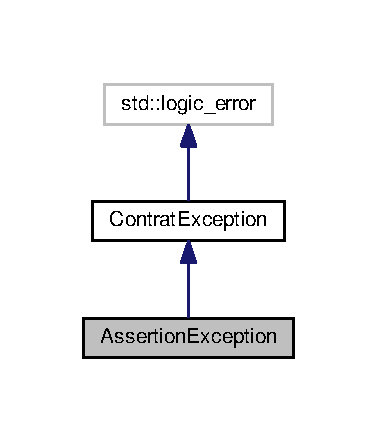
\includegraphics[width=181pt]{classAssertionException__inherit__graph}
\end{center}
\end{figure}


Collaboration diagram for Assertion\+Exception\+:\nopagebreak
\begin{figure}[H]
\begin{center}
\leavevmode
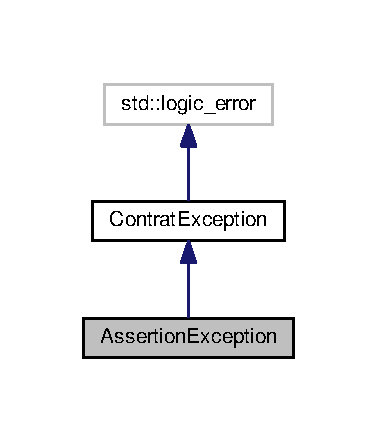
\includegraphics[width=181pt]{classAssertionException__coll__graph}
\end{center}
\end{figure}
\subsection*{Public Member Functions}
\begin{DoxyCompactItemize}
\item 
\hyperlink{classAssertionException_a93268f249b033bf4596901e50874fde6}{Assertion\+Exception} (std\+::string, unsigned int, std\+::string)
\begin{DoxyCompactList}\small\item\em Constructeur de la classe \hyperlink{classAssertionException}{Assertion\+Exception} ~\newline
 Le constructeur public \hyperlink{classAssertionException}{Assertion\+Exception}(...)initialise sa classe de base \hyperlink{classContratException}{Contrat\+Exception}. On n\textquotesingle{}a pas d\textquotesingle{}attribut local. Cette classe est intéressante pour son T\+Y\+PE lors du traitement des exceptions. \end{DoxyCompactList}\end{DoxyCompactItemize}


\subsection{Detailed Description}
Classe pour la gestion des erreurs d\textquotesingle{}assertion. 

\subsection{Constructor \& Destructor Documentation}
\index{Assertion\+Exception@{Assertion\+Exception}!Assertion\+Exception@{Assertion\+Exception}}
\index{Assertion\+Exception@{Assertion\+Exception}!Assertion\+Exception@{Assertion\+Exception}}
\subsubsection[{\texorpdfstring{Assertion\+Exception(std\+::string, unsigned int, std\+::string)}{AssertionException(std::string, unsigned int, std::string)}}]{\setlength{\rightskip}{0pt plus 5cm}Assertion\+Exception\+::\+Assertion\+Exception (
\begin{DoxyParamCaption}
\item[{std\+::string}]{p\+\_\+fichP, }
\item[{unsigned int}]{p\+\_\+prm\+Ligne, }
\item[{std\+::string}]{p\+\_\+exprP}
\end{DoxyParamCaption}
)}\hypertarget{classAssertionException_a93268f249b033bf4596901e50874fde6}{}\label{classAssertionException_a93268f249b033bf4596901e50874fde6}


Constructeur de la classe \hyperlink{classAssertionException}{Assertion\+Exception} ~\newline
 Le constructeur public \hyperlink{classAssertionException}{Assertion\+Exception}(...)initialise sa classe de base \hyperlink{classContratException}{Contrat\+Exception}. On n\textquotesingle{}a pas d\textquotesingle{}attribut local. Cette classe est intéressante pour son T\+Y\+PE lors du traitement des exceptions. 


\begin{DoxyParams}{Parameters}
{\em p\+\_\+fichP} & chaîne de caractères représentant le fichier source dans lequel a eu lieu l\textquotesingle{}erreur \\
\hline
{\em p\+\_\+prm\+Ligne} & un entier représentant la ligne où a eu lieu l\textquotesingle{}erreur \\
\hline
{\em p\+\_\+exprP} & Test logique qui a échoué \\
\hline
\end{DoxyParams}


The documentation for this class was generated from the following files\+:\begin{DoxyCompactItemize}
\item 
\hyperlink{ContratException_8h}{Contrat\+Exception.\+h}\item 
\hyperlink{ContratException_8cpp}{Contrat\+Exception.\+cpp}\end{DoxyCompactItemize}

\hypertarget{classbiblio_1_1Bibliographie}{}\section{biblio\+:\+:Bibliographie Class Reference}
\label{classbiblio_1_1Bibliographie}\index{biblio\+::\+Bibliographie@{biblio\+::\+Bibliographie}}


Classe \hyperlink{classbiblio_1_1Bibliographie}{Bibliographie}.  




{\ttfamily \#include $<$Bibliographie.\+h$>$}

\subsection*{Public Member Functions}
\begin{DoxyCompactItemize}
\item 
\hyperlink{classbiblio_1_1Bibliographie_a428979a1e88667d8dfc9ffb718a17dcf}{$\sim$\+Bibliographie} ()\hypertarget{classbiblio_1_1Bibliographie_a428979a1e88667d8dfc9ffb718a17dcf}{}\label{classbiblio_1_1Bibliographie_a428979a1e88667d8dfc9ffb718a17dcf}

\begin{DoxyCompactList}\small\item\em Un destructeur pour la classe \hyperlink{classbiblio_1_1Bibliographie}{Bibliographie}. \end{DoxyCompactList}\item 
\hyperlink{classbiblio_1_1Bibliographie_a04e86ad04d5e0510f7c6edd2c23358d6}{Bibliographie} (const std\+::string \&p\+\_\+nom)
\begin{DoxyCompactList}\small\item\em Constructeur de bibliographie pour donner un nom à la bibliographie. \end{DoxyCompactList}\item 
void \hyperlink{classbiblio_1_1Bibliographie_aa873f6c1a158c807072f91f3a5b33947}{ajouter\+Reference} (const \hyperlink{classbiblio_1_1Reference}{Reference} \&p\+\_\+nouvelle\+Reference)
\begin{DoxyCompactList}\small\item\em Méthode qui ajoute une référence formatée dans le vecteur reference. \end{DoxyCompactList}\item 
std\+::string \hyperlink{classbiblio_1_1Bibliographie_a6b503d643c36f9af56b3b85708e3bbe8}{req\+Bibliographie\+Formate} () const 
\begin{DoxyCompactList}\small\item\em Une méthode qui retourne une bibliographie formaté. \end{DoxyCompactList}\item 
const std\+::string \& {\bfseries req\+Nombiblio} () const \hypertarget{classbiblio_1_1Bibliographie_aeb99e2bdcde93a6eea2b30afabba7f26}{}\label{classbiblio_1_1Bibliographie_aeb99e2bdcde93a6eea2b30afabba7f26}

\end{DoxyCompactItemize}


\subsection{Detailed Description}
Classe \hyperlink{classbiblio_1_1Bibliographie}{Bibliographie}. 

\subsection{Constructor \& Destructor Documentation}
\index{biblio\+::\+Bibliographie@{biblio\+::\+Bibliographie}!Bibliographie@{Bibliographie}}
\index{Bibliographie@{Bibliographie}!biblio\+::\+Bibliographie@{biblio\+::\+Bibliographie}}
\subsubsection[{\texorpdfstring{Bibliographie(const std\+::string \&p\+\_\+nom)}{Bibliographie(const std::string &p_nom)}}]{\setlength{\rightskip}{0pt plus 5cm}biblio\+::\+Bibliographie\+::\+Bibliographie (
\begin{DoxyParamCaption}
\item[{const std\+::string \&}]{p\+\_\+nom}
\end{DoxyParamCaption}
)}\hypertarget{classbiblio_1_1Bibliographie_a04e86ad04d5e0510f7c6edd2c23358d6}{}\label{classbiblio_1_1Bibliographie_a04e86ad04d5e0510f7c6edd2c23358d6}


Constructeur de bibliographie pour donner un nom à la bibliographie. 


\begin{DoxyParams}{Parameters}
{\em p\+\_\+nom} & Nom de la bibliographie \\
\hline
\end{DoxyParams}


\subsection{Member Function Documentation}
\index{biblio\+::\+Bibliographie@{biblio\+::\+Bibliographie}!ajouter\+Reference@{ajouter\+Reference}}
\index{ajouter\+Reference@{ajouter\+Reference}!biblio\+::\+Bibliographie@{biblio\+::\+Bibliographie}}
\subsubsection[{\texorpdfstring{ajouter\+Reference(const Reference \&p\+\_\+nouvelle\+Reference)}{ajouterReference(const Reference &p_nouvelleReference)}}]{\setlength{\rightskip}{0pt plus 5cm}void biblio\+::\+Bibliographie\+::ajouter\+Reference (
\begin{DoxyParamCaption}
\item[{const {\bf Reference} \&}]{p\+\_\+nouvelle\+Reference}
\end{DoxyParamCaption}
)}\hypertarget{classbiblio_1_1Bibliographie_aa873f6c1a158c807072f91f3a5b33947}{}\label{classbiblio_1_1Bibliographie_aa873f6c1a158c807072f91f3a5b33947}


Méthode qui ajoute une référence formatée dans le vecteur reference. 


\begin{DoxyParams}{Parameters}
{\em p\+\_\+nouvelle\+Reference} & Nouvelle référence formaté. \\
\hline
\end{DoxyParams}
\index{biblio\+::\+Bibliographie@{biblio\+::\+Bibliographie}!req\+Bibliographie\+Formate@{req\+Bibliographie\+Formate}}
\index{req\+Bibliographie\+Formate@{req\+Bibliographie\+Formate}!biblio\+::\+Bibliographie@{biblio\+::\+Bibliographie}}
\subsubsection[{\texorpdfstring{req\+Bibliographie\+Formate() const }{reqBibliographieFormate() const }}]{\setlength{\rightskip}{0pt plus 5cm}string biblio\+::\+Bibliographie\+::req\+Bibliographie\+Formate (
\begin{DoxyParamCaption}
{}
\end{DoxyParamCaption}
) const}\hypertarget{classbiblio_1_1Bibliographie_a6b503d643c36f9af56b3b85708e3bbe8}{}\label{classbiblio_1_1Bibliographie_a6b503d643c36f9af56b3b85708e3bbe8}


Une méthode qui retourne une bibliographie formaté. 

\begin{DoxyReturn}{Returns}
os.\+str() La bibliographie formatée. 
\end{DoxyReturn}


The documentation for this class was generated from the following files\+:\begin{DoxyCompactItemize}
\item 
Bibliographie.\+h\item 
Bibliographie.\+cpp\end{DoxyCompactItemize}

\hypertarget{classContratException}{}\section{Contrat\+Exception Class Reference}
\label{classContratException}\index{Contrat\+Exception@{Contrat\+Exception}}


Classe de base des exceptions de contrat.  




{\ttfamily \#include $<$Contrat\+Exception.\+h$>$}



Inheritance diagram for Contrat\+Exception\+:\nopagebreak
\begin{figure}[H]
\begin{center}
\leavevmode
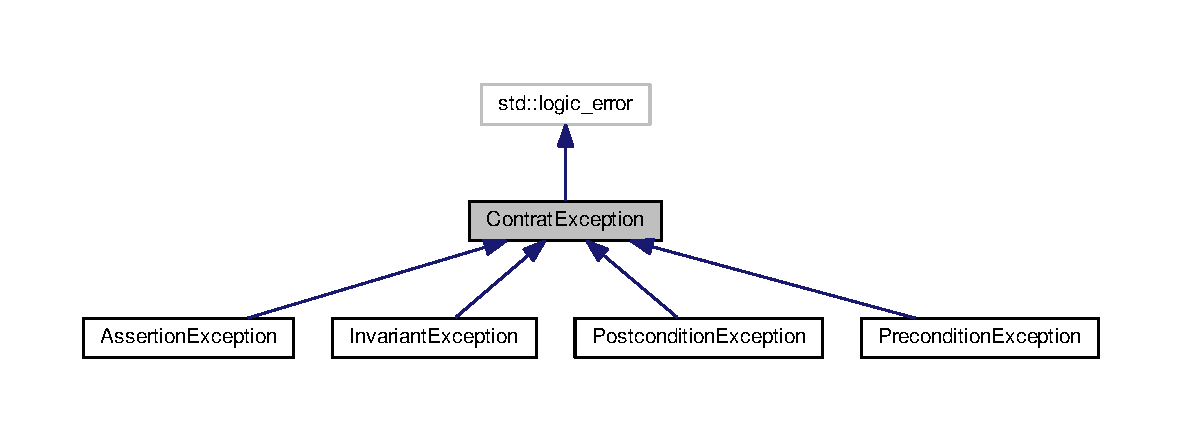
\includegraphics[width=350pt]{classContratException__inherit__graph}
\end{center}
\end{figure}


Collaboration diagram for Contrat\+Exception\+:\nopagebreak
\begin{figure}[H]
\begin{center}
\leavevmode
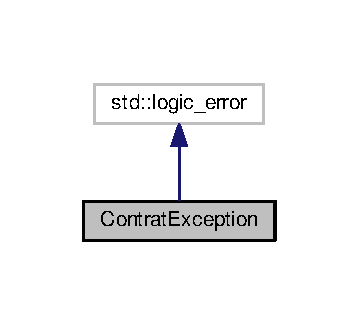
\includegraphics[width=172pt]{classContratException__coll__graph}
\end{center}
\end{figure}
\subsection*{Public Member Functions}
\begin{DoxyCompactItemize}
\item 
\hyperlink{classContratException_ad6c04fb577e960f87e010b125aa636a0}{Contrat\+Exception} (std\+::string, unsigned int, std\+::string, std\+::string)
\begin{DoxyCompactList}\small\item\em Constructeur de la classe de base \hyperlink{classContratException}{Contrat\+Exception}. \end{DoxyCompactList}\item 
std\+::string \hyperlink{classContratException_a8d20a9959f3b7cc4334165794dbaf1fc}{req\+Texte\+Exception} () const 
\begin{DoxyCompactList}\small\item\em Construit le texte complet relié à l\textquotesingle{}exception de contrat. \end{DoxyCompactList}\end{DoxyCompactItemize}


\subsection{Detailed Description}
Classe de base des exceptions de contrat. 

\subsection{Constructor \& Destructor Documentation}
\index{Contrat\+Exception@{Contrat\+Exception}!Contrat\+Exception@{Contrat\+Exception}}
\index{Contrat\+Exception@{Contrat\+Exception}!Contrat\+Exception@{Contrat\+Exception}}
\subsubsection[{\texorpdfstring{Contrat\+Exception(std\+::string, unsigned int, std\+::string, std\+::string)}{ContratException(std::string, unsigned int, std::string, std::string)}}]{\setlength{\rightskip}{0pt plus 5cm}Contrat\+Exception\+::\+Contrat\+Exception (
\begin{DoxyParamCaption}
\item[{std\+::string}]{p\+\_\+fichP, }
\item[{unsigned int}]{p\+\_\+prm\+Ligne, }
\item[{std\+::string}]{p\+\_\+exprP, }
\item[{std\+::string}]{p\+\_\+msgP}
\end{DoxyParamCaption}
)}\hypertarget{classContratException_ad6c04fb577e960f87e010b125aa636a0}{}\label{classContratException_ad6c04fb577e960f87e010b125aa636a0}


Constructeur de la classe de base \hyperlink{classContratException}{Contrat\+Exception}. 


\begin{DoxyParams}{Parameters}
{\em p\+\_\+fichP} & chaîne de caractères représentant le fichier source dans lequel a eu lieu l\textquotesingle{}erreur \\
\hline
{\em p\+\_\+prm\+Ligne} & un entier représentant la ligne où a eu lieu l\textquotesingle{}erreur \\
\hline
{\em p\+\_\+msgP} & Message décrivant l\textquotesingle{}erreur \\
\hline
{\em p\+\_\+exprP} & Test logique qui a échoué \\
\hline
\end{DoxyParams}


\subsection{Member Function Documentation}
\index{Contrat\+Exception@{Contrat\+Exception}!req\+Texte\+Exception@{req\+Texte\+Exception}}
\index{req\+Texte\+Exception@{req\+Texte\+Exception}!Contrat\+Exception@{Contrat\+Exception}}
\subsubsection[{\texorpdfstring{req\+Texte\+Exception() const }{reqTexteException() const }}]{\setlength{\rightskip}{0pt plus 5cm}std\+::string Contrat\+Exception\+::req\+Texte\+Exception (
\begin{DoxyParamCaption}
{}
\end{DoxyParamCaption}
) const}\hypertarget{classContratException_a8d20a9959f3b7cc4334165794dbaf1fc}{}\label{classContratException_a8d20a9959f3b7cc4334165794dbaf1fc}


Construit le texte complet relié à l\textquotesingle{}exception de contrat. 

\begin{DoxyReturn}{Returns}
une chaîne de caractères correspondant à l\textquotesingle{}exception 
\end{DoxyReturn}


The documentation for this class was generated from the following files\+:\begin{DoxyCompactItemize}
\item 
\hyperlink{ContratException_8h}{Contrat\+Exception.\+h}\item 
\hyperlink{ContratException_8cpp}{Contrat\+Exception.\+cpp}\end{DoxyCompactItemize}

\hypertarget{classInvariantException}{}\section{Invariant\+Exception Class Reference}
\label{classInvariantException}\index{Invariant\+Exception@{Invariant\+Exception}}


Classe pour la gestion des erreurs d\textquotesingle{}invariant.  




{\ttfamily \#include $<$Contrat\+Exception.\+h$>$}



Inheritance diagram for Invariant\+Exception\+:\nopagebreak
\begin{figure}[H]
\begin{center}
\leavevmode
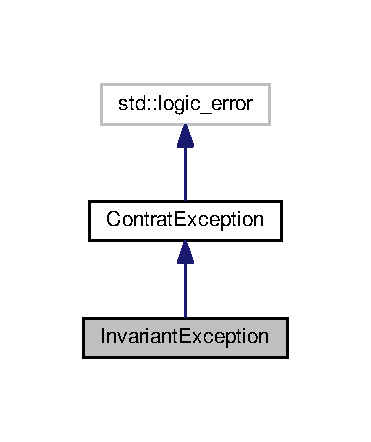
\includegraphics[width=178pt]{classInvariantException__inherit__graph}
\end{center}
\end{figure}


Collaboration diagram for Invariant\+Exception\+:\nopagebreak
\begin{figure}[H]
\begin{center}
\leavevmode
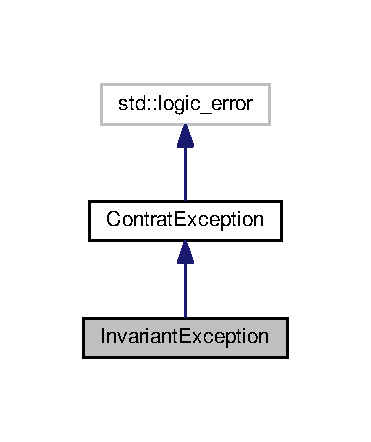
\includegraphics[width=178pt]{classInvariantException__coll__graph}
\end{center}
\end{figure}
\subsection*{Public Member Functions}
\begin{DoxyCompactItemize}
\item 
\hyperlink{classInvariantException_af8a1950834b26c256db0b11eb33e6056}{Invariant\+Exception} (std\+::string, unsigned int, std\+::string)
\begin{DoxyCompactList}\small\item\em Constructeur de la classe \hyperlink{classInvariantException}{Invariant\+Exception} en initialisant la classe de base \hyperlink{classContratException}{Contrat\+Exception}. La classe représente des erreurs d\textquotesingle{}invariant dans la théorie du contrat. \end{DoxyCompactList}\end{DoxyCompactItemize}


\subsection{Detailed Description}
Classe pour la gestion des erreurs d\textquotesingle{}invariant. 

\subsection{Constructor \& Destructor Documentation}
\index{Invariant\+Exception@{Invariant\+Exception}!Invariant\+Exception@{Invariant\+Exception}}
\index{Invariant\+Exception@{Invariant\+Exception}!Invariant\+Exception@{Invariant\+Exception}}
\subsubsection[{\texorpdfstring{Invariant\+Exception(std\+::string, unsigned int, std\+::string)}{InvariantException(std::string, unsigned int, std::string)}}]{\setlength{\rightskip}{0pt plus 5cm}Invariant\+Exception\+::\+Invariant\+Exception (
\begin{DoxyParamCaption}
\item[{std\+::string}]{p\+\_\+fichP, }
\item[{unsigned int}]{p\+\_\+prm\+Ligne, }
\item[{std\+::string}]{p\+\_\+exprP}
\end{DoxyParamCaption}
)}\hypertarget{classInvariantException_af8a1950834b26c256db0b11eb33e6056}{}\label{classInvariantException_af8a1950834b26c256db0b11eb33e6056}


Constructeur de la classe \hyperlink{classInvariantException}{Invariant\+Exception} en initialisant la classe de base \hyperlink{classContratException}{Contrat\+Exception}. La classe représente des erreurs d\textquotesingle{}invariant dans la théorie du contrat. 


\begin{DoxyParams}{Parameters}
{\em p\+\_\+fichP} & chaîne de caractères représentant le fichier source dans lequel a eu lieu l\textquotesingle{}erreur \\
\hline
{\em p\+\_\+prm\+Ligne} & un entier représentant la ligne où a eu lieu l\textquotesingle{}erreur \\
\hline
{\em p\+\_\+exprP} & Test logique qui a échoué \\
\hline
\end{DoxyParams}


The documentation for this class was generated from the following files\+:\begin{DoxyCompactItemize}
\item 
\hyperlink{ContratException_8h}{Contrat\+Exception.\+h}\item 
\hyperlink{ContratException_8cpp}{Contrat\+Exception.\+cpp}\end{DoxyCompactItemize}

\hypertarget{classJournal}{}\section{Journal Class Reference}
\label{classJournal}\index{Journal@{Journal}}


C\textquotesingle{}est la classe \hyperlink{classJournal}{Journal}.  




{\ttfamily \#include $<$Journal.\+h$>$}



\subsection{Detailed Description}
C\textquotesingle{}est la classe \hyperlink{classJournal}{Journal}. 

\hyperlink{Journal_8h_source}{Journal.\+h}

Created on\+: 2019-\/03-\/31 Author\+: Guillaume St-\/\+Georges 

The documentation for this class was generated from the following file\+:\begin{DoxyCompactItemize}
\item 
Journal.\+h\end{DoxyCompactItemize}

\hypertarget{classbiblio_1_1Journal}{}\section{biblio\+:\+:Journal Class Reference}
\label{classbiblio_1_1Journal}\index{biblio\+::\+Journal@{biblio\+::\+Journal}}


Inheritance diagram for biblio\+:\+:Journal\+:\nopagebreak
\begin{figure}[H]
\begin{center}
\leavevmode
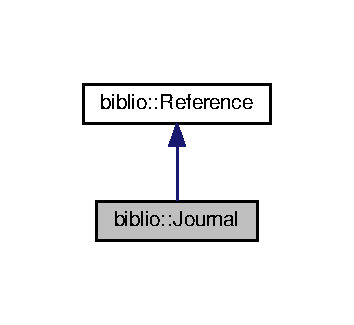
\includegraphics[width=170pt]{classbiblio_1_1Journal__inherit__graph}
\end{center}
\end{figure}


Collaboration diagram for biblio\+:\+:Journal\+:\nopagebreak
\begin{figure}[H]
\begin{center}
\leavevmode
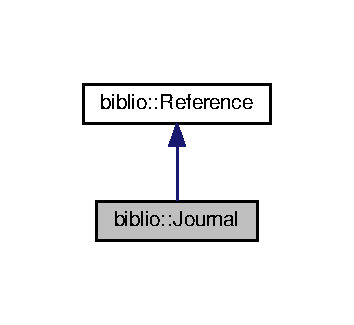
\includegraphics[width=170pt]{classbiblio_1_1Journal__coll__graph}
\end{center}
\end{figure}
\subsection*{Public Member Functions}
\begin{DoxyCompactItemize}
\item 
\hyperlink{classbiblio_1_1Journal_a0cb817e268b129cb1732ad8c4c2a9ccb}{$\sim$\+Journal} ()\hypertarget{classbiblio_1_1Journal_a0cb817e268b129cb1732ad8c4c2a9ccb}{}\label{classbiblio_1_1Journal_a0cb817e268b129cb1732ad8c4c2a9ccb}

\begin{DoxyCompactList}\small\item\em Destructeur de \hyperlink{classbiblio_1_1Journal}{Journal}. \end{DoxyCompactList}\item 
\hyperlink{classbiblio_1_1Journal_a83f03a7808ad679bdcaff8382c2ce718}{Journal} (std\+::string p\+\_\+auteurs, std\+::string p\+\_\+titre, int p\+\_\+annee, std\+::string p\+\_\+nom, int p\+\_\+volume, int p\+\_\+numero, int p\+\_\+page, std\+::string p\+\_\+identifiant)
\begin{DoxyCompactList}\small\item\em Contructeur qui crée un objet \hyperlink{classbiblio_1_1Journal}{Journal}. \end{DoxyCompactList}\item 
const std\+::string \& \hyperlink{classbiblio_1_1Journal_a224c3798a810bf334a47d3da1d58e42d}{req\+Nom} () const 
\begin{DoxyCompactList}\small\item\em Accesseur pour le nom du journal. \end{DoxyCompactList}\item 
int \hyperlink{classbiblio_1_1Journal_ab56f3828f03efefd102da330e3a0e543}{req\+Numero} () const 
\begin{DoxyCompactList}\small\item\em Accesseur pour le numéro du journal. \end{DoxyCompactList}\item 
int \hyperlink{classbiblio_1_1Journal_a7ed8914d6af79adf1d973665c544ea7d}{req\+Page} () const 
\begin{DoxyCompactList}\small\item\em Accesseur pour le nombre de pages. \end{DoxyCompactList}\item 
int \hyperlink{classbiblio_1_1Journal_a3a2d883971b4cc88754d20498f64a968}{req\+Volume} () const 
\begin{DoxyCompactList}\small\item\em Accesseur pour le numéro du volume du journal. \end{DoxyCompactList}\item 
std\+::string \hyperlink{classbiblio_1_1Journal_adb6c2688745a6a94fe62352b041def94}{req\+Reference\+Formate} () const 
\begin{DoxyCompactList}\small\item\em Formatteur de l\textquotesingle{}objet \hyperlink{classbiblio_1_1Journal}{Journal}. \end{DoxyCompactList}\item 
virtual \hyperlink{classbiblio_1_1Reference}{Reference} $\ast$ \hyperlink{classbiblio_1_1Journal_a74820672c820146f6b54a49ea0731958}{clone} () const 
\begin{DoxyCompactList}\small\item\em Clone de journal. \end{DoxyCompactList}\end{DoxyCompactItemize}


\subsection{Constructor \& Destructor Documentation}
\index{biblio\+::\+Journal@{biblio\+::\+Journal}!Journal@{Journal}}
\index{Journal@{Journal}!biblio\+::\+Journal@{biblio\+::\+Journal}}
\subsubsection[{\texorpdfstring{Journal(std\+::string p\+\_\+auteurs, std\+::string p\+\_\+titre, int p\+\_\+annee, std\+::string p\+\_\+nom, int p\+\_\+volume, int p\+\_\+numero, int p\+\_\+page, std\+::string p\+\_\+identifiant)}{Journal(std::string p_auteurs, std::string p_titre, int p_annee, std::string p_nom, int p_volume, int p_numero, int p_page, std::string p_identifiant)}}]{\setlength{\rightskip}{0pt plus 5cm}Journal\+::\+Journal (
\begin{DoxyParamCaption}
\item[{std\+::string}]{p\+\_\+auteurs, }
\item[{std\+::string}]{p\+\_\+titre, }
\item[{int}]{p\+\_\+annee, }
\item[{std\+::string}]{p\+\_\+nom, }
\item[{int}]{p\+\_\+volume, }
\item[{int}]{p\+\_\+numero, }
\item[{int}]{p\+\_\+page, }
\item[{std\+::string}]{p\+\_\+identifiant}
\end{DoxyParamCaption}
)}\hypertarget{classbiblio_1_1Journal_a83f03a7808ad679bdcaff8382c2ce718}{}\label{classbiblio_1_1Journal_a83f03a7808ad679bdcaff8382c2ce718}


Contructeur qui crée un objet \hyperlink{classbiblio_1_1Journal}{Journal}. 

\begin{DoxyPrecond}{Precondition}
Le journal doit avoir un nom 

Le volume commence à 1 

Le numéro doit être plus grand que 0 

Le nombre de pages doit être plus grand que 0 

L\textquotesingle{}identifiant doit être un code I\+S\+SN valide 
\end{DoxyPrecond}
\begin{DoxyPostcond}{Postcondition}
m\+\_\+nom doit être égal à p\+\_\+nom 

m\+\_\+volume doit être égal à p\+\_\+volume 

m\+\_\+numero doit être égal à p\+\_\+numero 

m\+\_\+page doit être égal à p\+\_\+page 
\end{DoxyPostcond}

\begin{DoxyParams}{Parameters}
{\em p\+\_\+auteurs} & Le nom des auteurs \\
\hline
{\em p\+\_\+titre} & Le titre de l\textquotesingle{}oeuvre \\
\hline
{\em p\+\_\+annee} & L\textquotesingle{}année d\textquotesingle{}édition \\
\hline
{\em p\+\_\+nom} & Le nom du journal \\
\hline
{\em p\+\_\+volume} & Le volume \\
\hline
{\em p\+\_\+numero} & Le numéro du volume \\
\hline
{\em p\+\_\+page} & Le nombre de pages \\
\hline
{\em p\+\_\+identifiant} & L\textquotesingle{}identifiant I\+S\+SN du journal \\
\hline
\end{DoxyParams}


\subsection{Member Function Documentation}
\index{biblio\+::\+Journal@{biblio\+::\+Journal}!clone@{clone}}
\index{clone@{clone}!biblio\+::\+Journal@{biblio\+::\+Journal}}
\subsubsection[{\texorpdfstring{clone() const }{clone() const }}]{\setlength{\rightskip}{0pt plus 5cm}{\bf Reference} $\ast$ Journal\+::clone (
\begin{DoxyParamCaption}
{}
\end{DoxyParamCaption}
) const\hspace{0.3cm}{\ttfamily [virtual]}}\hypertarget{classbiblio_1_1Journal_a74820672c820146f6b54a49ea0731958}{}\label{classbiblio_1_1Journal_a74820672c820146f6b54a49ea0731958}


Clone de journal. 

\begin{DoxyReturn}{Returns}
new \hyperlink{classJournal}{Journal($\ast$this)} Un clône de journal 
\end{DoxyReturn}


Implements \hyperlink{classbiblio_1_1Reference}{biblio\+::\+Reference}.

\index{biblio\+::\+Journal@{biblio\+::\+Journal}!req\+Nom@{req\+Nom}}
\index{req\+Nom@{req\+Nom}!biblio\+::\+Journal@{biblio\+::\+Journal}}
\subsubsection[{\texorpdfstring{req\+Nom() const }{reqNom() const }}]{\setlength{\rightskip}{0pt plus 5cm}const string \& Journal\+::req\+Nom (
\begin{DoxyParamCaption}
{}
\end{DoxyParamCaption}
) const}\hypertarget{classbiblio_1_1Journal_a224c3798a810bf334a47d3da1d58e42d}{}\label{classbiblio_1_1Journal_a224c3798a810bf334a47d3da1d58e42d}


Accesseur pour le nom du journal. 

\begin{DoxyReturn}{Returns}
m\+\_\+nom Le nom du journal 
\end{DoxyReturn}
\index{biblio\+::\+Journal@{biblio\+::\+Journal}!req\+Numero@{req\+Numero}}
\index{req\+Numero@{req\+Numero}!biblio\+::\+Journal@{biblio\+::\+Journal}}
\subsubsection[{\texorpdfstring{req\+Numero() const }{reqNumero() const }}]{\setlength{\rightskip}{0pt plus 5cm}int Journal\+::req\+Numero (
\begin{DoxyParamCaption}
{}
\end{DoxyParamCaption}
) const}\hypertarget{classbiblio_1_1Journal_ab56f3828f03efefd102da330e3a0e543}{}\label{classbiblio_1_1Journal_ab56f3828f03efefd102da330e3a0e543}


Accesseur pour le numéro du journal. 

\begin{DoxyReturn}{Returns}
m\+\_\+numero Le numéro du journal 
\end{DoxyReturn}
\index{biblio\+::\+Journal@{biblio\+::\+Journal}!req\+Page@{req\+Page}}
\index{req\+Page@{req\+Page}!biblio\+::\+Journal@{biblio\+::\+Journal}}
\subsubsection[{\texorpdfstring{req\+Page() const }{reqPage() const }}]{\setlength{\rightskip}{0pt plus 5cm}int Journal\+::req\+Page (
\begin{DoxyParamCaption}
{}
\end{DoxyParamCaption}
) const}\hypertarget{classbiblio_1_1Journal_a7ed8914d6af79adf1d973665c544ea7d}{}\label{classbiblio_1_1Journal_a7ed8914d6af79adf1d973665c544ea7d}


Accesseur pour le nombre de pages. 

\begin{DoxyReturn}{Returns}
m\+\_\+page Le nombre de pages du journal 
\end{DoxyReturn}
\index{biblio\+::\+Journal@{biblio\+::\+Journal}!req\+Reference\+Formate@{req\+Reference\+Formate}}
\index{req\+Reference\+Formate@{req\+Reference\+Formate}!biblio\+::\+Journal@{biblio\+::\+Journal}}
\subsubsection[{\texorpdfstring{req\+Reference\+Formate() const }{reqReferenceFormate() const }}]{\setlength{\rightskip}{0pt plus 5cm}std\+::string Journal\+::req\+Reference\+Formate (
\begin{DoxyParamCaption}
{}
\end{DoxyParamCaption}
) const\hspace{0.3cm}{\ttfamily [virtual]}}\hypertarget{classbiblio_1_1Journal_adb6c2688745a6a94fe62352b041def94}{}\label{classbiblio_1_1Journal_adb6c2688745a6a94fe62352b041def94}


Formatteur de l\textquotesingle{}objet \hyperlink{classbiblio_1_1Journal}{Journal}. 

\begin{DoxyReturn}{Returns}

\end{DoxyReturn}


Implements \hyperlink{classbiblio_1_1Reference_a6a1a403b66587341f89aca0e9d6c4f7a}{biblio\+::\+Reference}.

\index{biblio\+::\+Journal@{biblio\+::\+Journal}!req\+Volume@{req\+Volume}}
\index{req\+Volume@{req\+Volume}!biblio\+::\+Journal@{biblio\+::\+Journal}}
\subsubsection[{\texorpdfstring{req\+Volume() const }{reqVolume() const }}]{\setlength{\rightskip}{0pt plus 5cm}int Journal\+::req\+Volume (
\begin{DoxyParamCaption}
{}
\end{DoxyParamCaption}
) const}\hypertarget{classbiblio_1_1Journal_a3a2d883971b4cc88754d20498f64a968}{}\label{classbiblio_1_1Journal_a3a2d883971b4cc88754d20498f64a968}


Accesseur pour le numéro du volume du journal. 

\begin{DoxyReturn}{Returns}
m\+\_\+volume Le numéro du volume du journal 
\end{DoxyReturn}


The documentation for this class was generated from the following files\+:\begin{DoxyCompactItemize}
\item 
Journal.\+h\item 
Journal.\+cpp\end{DoxyCompactItemize}

\hypertarget{classbiblio_1_1Ouvrage}{}\section{biblio\+:\+:Ouvrage Class Reference}
\label{classbiblio_1_1Ouvrage}\index{biblio\+::\+Ouvrage@{biblio\+::\+Ouvrage}}


Classe \hyperlink{classbiblio_1_1Ouvrage}{Ouvrage}.  




{\ttfamily \#include $<$Ouvrage.\+h$>$}



Inheritance diagram for biblio\+:\+:Ouvrage\+:\nopagebreak
\begin{figure}[H]
\begin{center}
\leavevmode
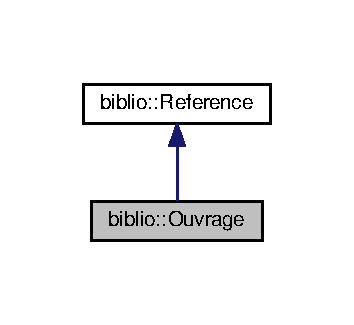
\includegraphics[width=170pt]{classbiblio_1_1Ouvrage__inherit__graph}
\end{center}
\end{figure}


Collaboration diagram for biblio\+:\+:Ouvrage\+:\nopagebreak
\begin{figure}[H]
\begin{center}
\leavevmode
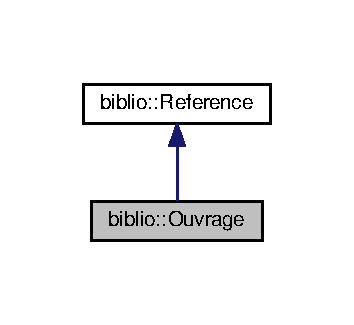
\includegraphics[width=170pt]{classbiblio_1_1Ouvrage__coll__graph}
\end{center}
\end{figure}
\subsection*{Public Member Functions}
\begin{DoxyCompactItemize}
\item 
\hyperlink{classbiblio_1_1Ouvrage_ac3c4cb2c73e6382eb6760297bdace9e7}{Ouvrage} (std\+::string p\+\_\+auteurs, std\+::string p\+\_\+titre, std\+::string p\+\_\+editeur, std\+::string p\+\_\+ville, int p\+\_\+annee, std\+::string p\+\_\+identifiant)
\begin{DoxyCompactList}\small\item\em Constructeur qui crée un objet \hyperlink{classbiblio_1_1Ouvrage}{Ouvrage}. \end{DoxyCompactList}\item 
const std\+::string \& \hyperlink{classbiblio_1_1Ouvrage_ae1d95d392ad151ef64dfcc7742e741df}{req\+Editeur} () const 
\begin{DoxyCompactList}\small\item\em Accessseur pour l\textquotesingle{}éditeur. \end{DoxyCompactList}\item 
const std\+::string \& \hyperlink{classbiblio_1_1Ouvrage_a7d376d2d74056e00dfdc38d7626575be}{req\+Ville} () const 
\begin{DoxyCompactList}\small\item\em Accessseur pour la ville. \end{DoxyCompactList}\item 
std\+::string \hyperlink{classbiblio_1_1Ouvrage_afe9e9c3ca248578c1799bd3bce528835}{req\+Reference\+Formate} () const 
\begin{DoxyCompactList}\small\item\em Une méthode pour formater un objet \hyperlink{classbiblio_1_1Ouvrage}{Ouvrage}. \end{DoxyCompactList}\item 
virtual \hyperlink{classbiblio_1_1Reference}{Reference} $\ast$ \hyperlink{classbiblio_1_1Ouvrage_a3c79215a9af35ef05d1d89ba25ae21bb}{clone} () const 
\begin{DoxyCompactList}\small\item\em Une méthode qui clone un objet \hyperlink{classbiblio_1_1Ouvrage}{Ouvrage}. \end{DoxyCompactList}\end{DoxyCompactItemize}


\subsection{Detailed Description}
Classe \hyperlink{classbiblio_1_1Ouvrage}{Ouvrage}. 

\subsection{Constructor \& Destructor Documentation}
\index{biblio\+::\+Ouvrage@{biblio\+::\+Ouvrage}!Ouvrage@{Ouvrage}}
\index{Ouvrage@{Ouvrage}!biblio\+::\+Ouvrage@{biblio\+::\+Ouvrage}}
\subsubsection[{\texorpdfstring{Ouvrage(std\+::string p\+\_\+auteurs, std\+::string p\+\_\+titre, std\+::string p\+\_\+editeur, std\+::string p\+\_\+ville, int p\+\_\+annee, std\+::string p\+\_\+identifiant)}{Ouvrage(std::string p_auteurs, std::string p_titre, std::string p_editeur, std::string p_ville, int p_annee, std::string p_identifiant)}}]{\setlength{\rightskip}{0pt plus 5cm}biblio\+::\+Ouvrage\+::\+Ouvrage (
\begin{DoxyParamCaption}
\item[{std\+::string}]{p\+\_\+auteurs, }
\item[{std\+::string}]{p\+\_\+titre, }
\item[{std\+::string}]{p\+\_\+editeur, }
\item[{std\+::string}]{p\+\_\+ville, }
\item[{int}]{p\+\_\+annee, }
\item[{std\+::string}]{p\+\_\+identifiant}
\end{DoxyParamCaption}
)}\hypertarget{classbiblio_1_1Ouvrage_ac3c4cb2c73e6382eb6760297bdace9e7}{}\label{classbiblio_1_1Ouvrage_ac3c4cb2c73e6382eb6760297bdace9e7}


Constructeur qui crée un objet \hyperlink{classbiblio_1_1Ouvrage}{Ouvrage}. 

\begin{DoxyPrecond}{Precondition}
p\+\_\+editeur doit être dans un format valide 

p\+\_\+ville doit être dans un format valide 
\end{DoxyPrecond}
\begin{DoxyPostcond}{Postcondition}
m\+\_\+editeur doit être égal à p\+\_\+editeur 

m\+\_\+ville doit être égal à p\+\_\+ville 
\end{DoxyPostcond}

\begin{DoxyParams}{Parameters}
{\em p\+\_\+editeur} & \\
\hline
{\em p\+\_\+ville} & \\
\hline
\end{DoxyParams}
\begin{DoxyReturn}{Returns}
un objet \hyperlink{classbiblio_1_1Ouvrage}{Ouvrage} 
\end{DoxyReturn}


\subsection{Member Function Documentation}
\index{biblio\+::\+Ouvrage@{biblio\+::\+Ouvrage}!clone@{clone}}
\index{clone@{clone}!biblio\+::\+Ouvrage@{biblio\+::\+Ouvrage}}
\subsubsection[{\texorpdfstring{clone() const }{clone() const }}]{\setlength{\rightskip}{0pt plus 5cm}{\bf Reference} $\ast$ biblio\+::\+Ouvrage\+::clone (
\begin{DoxyParamCaption}
{}
\end{DoxyParamCaption}
) const\hspace{0.3cm}{\ttfamily [virtual]}}\hypertarget{classbiblio_1_1Ouvrage_a3c79215a9af35ef05d1d89ba25ae21bb}{}\label{classbiblio_1_1Ouvrage_a3c79215a9af35ef05d1d89ba25ae21bb}


Une méthode qui clone un objet \hyperlink{classbiblio_1_1Ouvrage}{Ouvrage}. 

\begin{DoxyReturn}{Returns}
new Ouvrage($\ast$this) Un clône de l\textquotesingle{}objet \hyperlink{classbiblio_1_1Ouvrage}{Ouvrage}. 
\end{DoxyReturn}


Implements \hyperlink{classbiblio_1_1Reference}{biblio\+::\+Reference}.

\index{biblio\+::\+Ouvrage@{biblio\+::\+Ouvrage}!req\+Editeur@{req\+Editeur}}
\index{req\+Editeur@{req\+Editeur}!biblio\+::\+Ouvrage@{biblio\+::\+Ouvrage}}
\subsubsection[{\texorpdfstring{req\+Editeur() const }{reqEditeur() const }}]{\setlength{\rightskip}{0pt plus 5cm}const string \& biblio\+::\+Ouvrage\+::req\+Editeur (
\begin{DoxyParamCaption}
{}
\end{DoxyParamCaption}
) const}\hypertarget{classbiblio_1_1Ouvrage_ae1d95d392ad151ef64dfcc7742e741df}{}\label{classbiblio_1_1Ouvrage_ae1d95d392ad151ef64dfcc7742e741df}


Accessseur pour l\textquotesingle{}éditeur. 

\begin{DoxyReturn}{Returns}
m\+\_\+editeur L\textquotesingle{}éditeur de la classe \hyperlink{classbiblio_1_1Ouvrage}{Ouvrage} 
\end{DoxyReturn}
\index{biblio\+::\+Ouvrage@{biblio\+::\+Ouvrage}!req\+Reference\+Formate@{req\+Reference\+Formate}}
\index{req\+Reference\+Formate@{req\+Reference\+Formate}!biblio\+::\+Ouvrage@{biblio\+::\+Ouvrage}}
\subsubsection[{\texorpdfstring{req\+Reference\+Formate() const }{reqReferenceFormate() const }}]{\setlength{\rightskip}{0pt plus 5cm}std\+::string biblio\+::\+Ouvrage\+::req\+Reference\+Formate (
\begin{DoxyParamCaption}
{}
\end{DoxyParamCaption}
) const\hspace{0.3cm}{\ttfamily [virtual]}}\hypertarget{classbiblio_1_1Ouvrage_afe9e9c3ca248578c1799bd3bce528835}{}\label{classbiblio_1_1Ouvrage_afe9e9c3ca248578c1799bd3bce528835}


Une méthode pour formater un objet \hyperlink{classbiblio_1_1Ouvrage}{Ouvrage}. 

\begin{DoxyReturn}{Returns}
os.\+str() Un objet \hyperlink{classbiblio_1_1Ouvrage}{Ouvrage} formaté 
\end{DoxyReturn}


Implements \hyperlink{classbiblio_1_1Reference_a6a1a403b66587341f89aca0e9d6c4f7a}{biblio\+::\+Reference}.

\index{biblio\+::\+Ouvrage@{biblio\+::\+Ouvrage}!req\+Ville@{req\+Ville}}
\index{req\+Ville@{req\+Ville}!biblio\+::\+Ouvrage@{biblio\+::\+Ouvrage}}
\subsubsection[{\texorpdfstring{req\+Ville() const }{reqVille() const }}]{\setlength{\rightskip}{0pt plus 5cm}const string \& biblio\+::\+Ouvrage\+::req\+Ville (
\begin{DoxyParamCaption}
{}
\end{DoxyParamCaption}
) const}\hypertarget{classbiblio_1_1Ouvrage_a7d376d2d74056e00dfdc38d7626575be}{}\label{classbiblio_1_1Ouvrage_a7d376d2d74056e00dfdc38d7626575be}


Accessseur pour la ville. 

\begin{DoxyReturn}{Returns}
m\+\_\+ville La ville de la classe \hyperlink{classbiblio_1_1Ouvrage}{Ouvrage} 
\end{DoxyReturn}


The documentation for this class was generated from the following files\+:\begin{DoxyCompactItemize}
\item 
Ouvrage.\+h\item 
Ouvrage.\+cpp\end{DoxyCompactItemize}

\hypertarget{classPostconditionException}{}\section{Postcondition\+Exception Class Reference}
\label{classPostconditionException}\index{Postcondition\+Exception@{Postcondition\+Exception}}


Classe pour la gestion des erreurs de postcondition.  




{\ttfamily \#include $<$Contrat\+Exception.\+h$>$}



Inheritance diagram for Postcondition\+Exception\+:\nopagebreak
\begin{figure}[H]
\begin{center}
\leavevmode
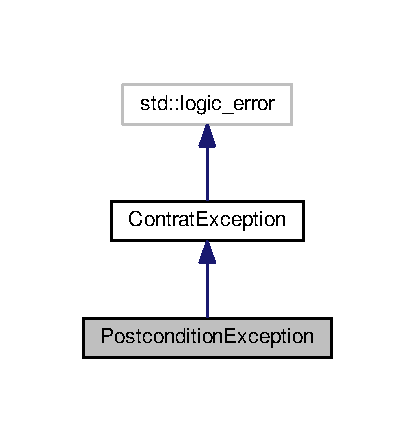
\includegraphics[width=199pt]{classPostconditionException__inherit__graph}
\end{center}
\end{figure}


Collaboration diagram for Postcondition\+Exception\+:\nopagebreak
\begin{figure}[H]
\begin{center}
\leavevmode
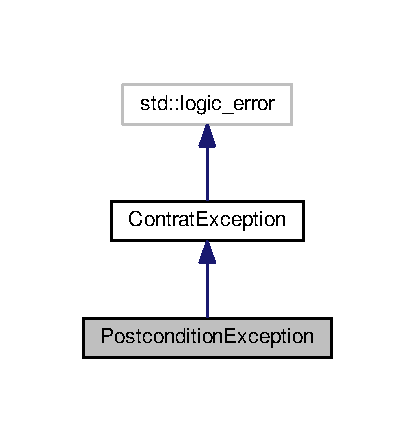
\includegraphics[width=199pt]{classPostconditionException__coll__graph}
\end{center}
\end{figure}
\subsection*{Public Member Functions}
\begin{DoxyCompactItemize}
\item 
\hyperlink{classPostconditionException_acc95ea17c4302b996261b7201d2cf6c4}{Postcondition\+Exception} (std\+::string, unsigned int, std\+::string)
\begin{DoxyCompactList}\small\item\em Constructeur de la classe \hyperlink{classPostconditionException}{Postcondition\+Exception} en initialisant la classe de base \hyperlink{classContratException}{Contrat\+Exception}. La classe représente des erreurs de postcondition dans la théorie du contrat. \end{DoxyCompactList}\end{DoxyCompactItemize}


\subsection{Detailed Description}
Classe pour la gestion des erreurs de postcondition. 

\subsection{Constructor \& Destructor Documentation}
\index{Postcondition\+Exception@{Postcondition\+Exception}!Postcondition\+Exception@{Postcondition\+Exception}}
\index{Postcondition\+Exception@{Postcondition\+Exception}!Postcondition\+Exception@{Postcondition\+Exception}}
\subsubsection[{\texorpdfstring{Postcondition\+Exception(std\+::string, unsigned int, std\+::string)}{PostconditionException(std::string, unsigned int, std::string)}}]{\setlength{\rightskip}{0pt plus 5cm}Postcondition\+Exception\+::\+Postcondition\+Exception (
\begin{DoxyParamCaption}
\item[{std\+::string}]{p\+\_\+fichP, }
\item[{unsigned int}]{p\+\_\+prm\+Ligne, }
\item[{std\+::string}]{p\+\_\+exprP}
\end{DoxyParamCaption}
)}\hypertarget{classPostconditionException_acc95ea17c4302b996261b7201d2cf6c4}{}\label{classPostconditionException_acc95ea17c4302b996261b7201d2cf6c4}


Constructeur de la classe \hyperlink{classPostconditionException}{Postcondition\+Exception} en initialisant la classe de base \hyperlink{classContratException}{Contrat\+Exception}. La classe représente des erreurs de postcondition dans la théorie du contrat. 


\begin{DoxyParams}{Parameters}
{\em p\+\_\+fichP} & chaîne de caractères représentant le fichier source dans lequel a eu lieu l\textquotesingle{}erreur \\
\hline
{\em p\+\_\+prm\+Ligne} & un entier représentant la ligne où a eu lieu l\textquotesingle{}erreur \\
\hline
{\em p\+\_\+exprP} & Test logique qui a échoué \\
\hline
\end{DoxyParams}


The documentation for this class was generated from the following files\+:\begin{DoxyCompactItemize}
\item 
\hyperlink{ContratException_8h}{Contrat\+Exception.\+h}\item 
\hyperlink{ContratException_8cpp}{Contrat\+Exception.\+cpp}\end{DoxyCompactItemize}

\hypertarget{classPreconditionException}{}\section{Precondition\+Exception Class Reference}
\label{classPreconditionException}\index{Precondition\+Exception@{Precondition\+Exception}}


Classe pour la gestion des erreurs de précondition.  




{\ttfamily \#include $<$Contrat\+Exception.\+h$>$}



Inheritance diagram for Precondition\+Exception\+:\nopagebreak
\begin{figure}[H]
\begin{center}
\leavevmode
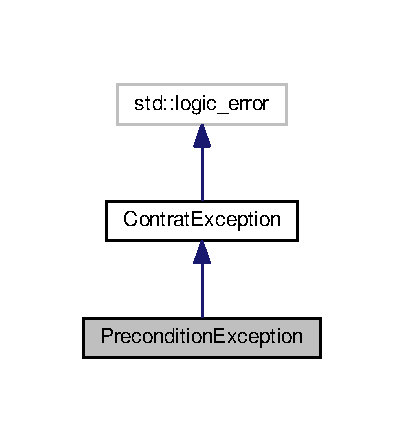
\includegraphics[width=194pt]{classPreconditionException__inherit__graph}
\end{center}
\end{figure}


Collaboration diagram for Precondition\+Exception\+:\nopagebreak
\begin{figure}[H]
\begin{center}
\leavevmode
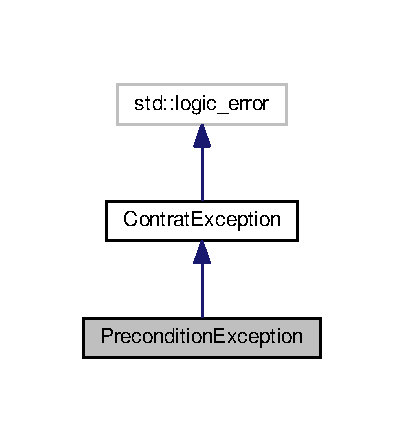
\includegraphics[width=194pt]{classPreconditionException__coll__graph}
\end{center}
\end{figure}
\subsection*{Public Member Functions}
\begin{DoxyCompactItemize}
\item 
\hyperlink{classPreconditionException_a66d4b4c57a0675d487dab85d2c31b08c}{Precondition\+Exception} (std\+::string, unsigned int, std\+::string)
\begin{DoxyCompactList}\small\item\em Constructeur de la classe \hyperlink{classPreconditionException}{Precondition\+Exception} en initialisant la classe de base \hyperlink{classContratException}{Contrat\+Exception}. La classe représente l\textquotesingle{}erreur de précondition dans la théorie du contrat. \end{DoxyCompactList}\end{DoxyCompactItemize}


\subsection{Detailed Description}
Classe pour la gestion des erreurs de précondition. 

\subsection{Constructor \& Destructor Documentation}
\index{Precondition\+Exception@{Precondition\+Exception}!Precondition\+Exception@{Precondition\+Exception}}
\index{Precondition\+Exception@{Precondition\+Exception}!Precondition\+Exception@{Precondition\+Exception}}
\subsubsection[{\texorpdfstring{Precondition\+Exception(std\+::string, unsigned int, std\+::string)}{PreconditionException(std::string, unsigned int, std::string)}}]{\setlength{\rightskip}{0pt plus 5cm}Precondition\+Exception\+::\+Precondition\+Exception (
\begin{DoxyParamCaption}
\item[{std\+::string}]{p\+\_\+fichP, }
\item[{unsigned int}]{p\+\_\+prm\+Ligne, }
\item[{std\+::string}]{p\+\_\+exprP}
\end{DoxyParamCaption}
)}\hypertarget{classPreconditionException_a66d4b4c57a0675d487dab85d2c31b08c}{}\label{classPreconditionException_a66d4b4c57a0675d487dab85d2c31b08c}


Constructeur de la classe \hyperlink{classPreconditionException}{Precondition\+Exception} en initialisant la classe de base \hyperlink{classContratException}{Contrat\+Exception}. La classe représente l\textquotesingle{}erreur de précondition dans la théorie du contrat. 


\begin{DoxyParams}{Parameters}
{\em p\+\_\+fichP} & chaîne de caractères représentant le fichier source dans lequel a eu lieu l\textquotesingle{}erreur \\
\hline
{\em p\+\_\+prm\+Ligne} & un entier représentant la ligne où a eu lieu l\textquotesingle{}erreur \\
\hline
{\em p\+\_\+exprP} & Test logique qui a échoué \\
\hline
\end{DoxyParams}


The documentation for this class was generated from the following files\+:\begin{DoxyCompactItemize}
\item 
\hyperlink{ContratException_8h}{Contrat\+Exception.\+h}\item 
\hyperlink{ContratException_8cpp}{Contrat\+Exception.\+cpp}\end{DoxyCompactItemize}

\hypertarget{classbiblio_1_1Reference}{}\section{biblio\+:\+:Reference Class Reference}
\label{classbiblio_1_1Reference}\index{biblio\+::\+Reference@{biblio\+::\+Reference}}


Classe \hyperlink{classbiblio_1_1Reference}{Reference} permettant de modéliser les objets reference.  




{\ttfamily \#include $<$Reference.\+h$>$}



Inheritance diagram for biblio\+:\+:Reference\+:\nopagebreak
\begin{figure}[H]
\begin{center}
\leavevmode
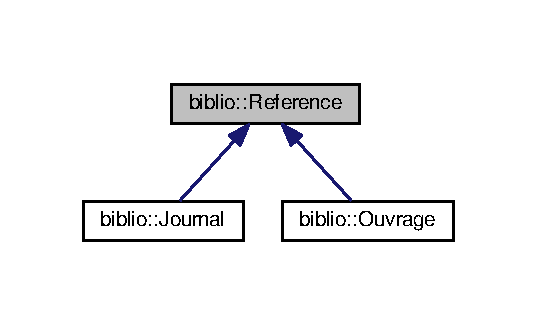
\includegraphics[width=257pt]{classbiblio_1_1Reference__inherit__graph}
\end{center}
\end{figure}
\subsection*{Public Member Functions}
\begin{DoxyCompactItemize}
\item 
{\bfseries Reference} (std\+::string p\+\_\+auteurs, std\+::string p\+\_\+titre, int p\+\_\+annee, std\+::string p\+\_\+identifiant)\hypertarget{classbiblio_1_1Reference_a9b67b87dbb52b8aed293fff4b8184c5e}{}\label{classbiblio_1_1Reference_a9b67b87dbb52b8aed293fff4b8184c5e}

\item 
int \hyperlink{classbiblio_1_1Reference_acaa3e9f6b56c94a13374de5ce7984d30}{req\+Annee} () const 
\begin{DoxyCompactList}\small\item\em Accesseur pour l\textquotesingle{}année. \end{DoxyCompactList}\item 
const std\+::string \& \hyperlink{classbiblio_1_1Reference_a5ab6c05f95be3beb7591c588413ac6bf}{req\+Auteurs} () const 
\begin{DoxyCompactList}\small\item\em Accesseur pour le/les auteurs. \end{DoxyCompactList}\item 
void \hyperlink{classbiblio_1_1Reference_aee041fbf9b44e02241eb717783a5d8f2}{asg\+Auteurs} (const std\+::string \&p\+\_\+auteurs)
\begin{DoxyCompactList}\small\item\em des auteurs \end{DoxyCompactList}\item 
const std\+::string \& \hyperlink{classbiblio_1_1Reference_a2b00f5c1e762abee52ba30bb3fbfab37}{req\+Identifiant} () const 
\begin{DoxyCompactList}\small\item\em Assigneur d\textquotesingle{}identifiant. \end{DoxyCompactList}\item 
const std\+::string \& \hyperlink{classbiblio_1_1Reference_acc2a2075747a2e26f0d4eaab742f4f31}{req\+Titre} () const 
\begin{DoxyCompactList}\small\item\em Assigneur de titre. \end{DoxyCompactList}\item 
virtual std\+::string \hyperlink{classbiblio_1_1Reference_a6a1a403b66587341f89aca0e9d6c4f7a}{req\+Reference\+Formate} () const =0
\item 
bool \hyperlink{classbiblio_1_1Reference_a48220b30f6704d6f0aca13bf51022375}{operator==} (const \hyperlink{classbiblio_1_1Reference}{Reference} \&ref) const 
\item 
virtual \hyperlink{classbiblio_1_1Reference}{Reference} $\ast$ {\bfseries clone} () const =0\hypertarget{classbiblio_1_1Reference_a912da874b8a5221d8e17aa3118d3116b}{}\label{classbiblio_1_1Reference_a912da874b8a5221d8e17aa3118d3116b}

\end{DoxyCompactItemize}


\subsection{Detailed Description}
Classe \hyperlink{classbiblio_1_1Reference}{Reference} permettant de modéliser les objets reference. 

\subsection{Member Function Documentation}
\index{biblio\+::\+Reference@{biblio\+::\+Reference}!asg\+Auteurs@{asg\+Auteurs}}
\index{asg\+Auteurs@{asg\+Auteurs}!biblio\+::\+Reference@{biblio\+::\+Reference}}
\subsubsection[{\texorpdfstring{asg\+Auteurs(const std\+::string \&p\+\_\+auteurs)}{asgAuteurs(const std::string &p_auteurs)}}]{\setlength{\rightskip}{0pt plus 5cm}void biblio\+::\+Reference\+::asg\+Auteurs (
\begin{DoxyParamCaption}
\item[{const std\+::string \&}]{p\+\_\+auteurs}
\end{DoxyParamCaption}
)}\hypertarget{classbiblio_1_1Reference_aee041fbf9b44e02241eb717783a5d8f2}{}\label{classbiblio_1_1Reference_aee041fbf9b44e02241eb717783a5d8f2}


des auteurs 


\begin{DoxyParams}[1]{Parameters}
\mbox{\tt in}  & {\em p\+\_\+auteurs} & Les noms des auteurs \\
\hline
\end{DoxyParams}
\index{biblio\+::\+Reference@{biblio\+::\+Reference}!operator==@{operator==}}
\index{operator==@{operator==}!biblio\+::\+Reference@{biblio\+::\+Reference}}
\subsubsection[{\texorpdfstring{operator==(const Reference \&ref) const }{operator==(const Reference &ref) const }}]{\setlength{\rightskip}{0pt plus 5cm}bool biblio\+::\+Reference\+::operator== (
\begin{DoxyParamCaption}
\item[{const {\bf Reference} \&}]{ref}
\end{DoxyParamCaption}
) const}\hypertarget{classbiblio_1_1Reference_a48220b30f6704d6f0aca13bf51022375}{}\label{classbiblio_1_1Reference_a48220b30f6704d6f0aca13bf51022375}

\begin{DoxyParams}[1]{Parameters}
\mbox{\tt in}  & {\em ref} & Un objet de la classe \hyperlink{classbiblio_1_1Reference}{Reference} \\
\hline
\end{DoxyParams}
\begin{DoxyReturn}{Returns}
m\+\_\+auteurs == ref.\+m\+\_\+auteurs \&\& m\+\_\+titre == ref.\+m\+\_\+titre \&\& m\+\_\+annee == ref.\+m\+\_\+annee \&\& m\+\_\+identifiant == ref.\+m\+\_\+identifiant Des opérateurs logiques d\textquotesingle{}égalité 
\end{DoxyReturn}
\index{biblio\+::\+Reference@{biblio\+::\+Reference}!req\+Annee@{req\+Annee}}
\index{req\+Annee@{req\+Annee}!biblio\+::\+Reference@{biblio\+::\+Reference}}
\subsubsection[{\texorpdfstring{req\+Annee() const }{reqAnnee() const }}]{\setlength{\rightskip}{0pt plus 5cm}int biblio\+::\+Reference\+::req\+Annee (
\begin{DoxyParamCaption}
{}
\end{DoxyParamCaption}
) const}\hypertarget{classbiblio_1_1Reference_acaa3e9f6b56c94a13374de5ce7984d30}{}\label{classbiblio_1_1Reference_acaa3e9f6b56c94a13374de5ce7984d30}


Accesseur pour l\textquotesingle{}année. 


\begin{DoxyParams}[1]{Parameters}
\mbox{\tt in}  & {\em m\+\_\+annee} & L\textquotesingle{}année de référence \\
\hline
\end{DoxyParams}
\begin{DoxyReturn}{Returns}
m\+\_\+annee L\textquotesingle{}année de référence 
\end{DoxyReturn}
\index{biblio\+::\+Reference@{biblio\+::\+Reference}!req\+Auteurs@{req\+Auteurs}}
\index{req\+Auteurs@{req\+Auteurs}!biblio\+::\+Reference@{biblio\+::\+Reference}}
\subsubsection[{\texorpdfstring{req\+Auteurs() const }{reqAuteurs() const }}]{\setlength{\rightskip}{0pt plus 5cm}const std\+::string \& biblio\+::\+Reference\+::req\+Auteurs (
\begin{DoxyParamCaption}
{}
\end{DoxyParamCaption}
) const}\hypertarget{classbiblio_1_1Reference_a5ab6c05f95be3beb7591c588413ac6bf}{}\label{classbiblio_1_1Reference_a5ab6c05f95be3beb7591c588413ac6bf}


Accesseur pour le/les auteurs. 

\begin{DoxyReturn}{Returns}
m\+\_\+auteurs Le(s) nom(s) de l\textquotesingle{}auteur ou des auteurs 
\end{DoxyReturn}
\index{biblio\+::\+Reference@{biblio\+::\+Reference}!req\+Identifiant@{req\+Identifiant}}
\index{req\+Identifiant@{req\+Identifiant}!biblio\+::\+Reference@{biblio\+::\+Reference}}
\subsubsection[{\texorpdfstring{req\+Identifiant() const }{reqIdentifiant() const }}]{\setlength{\rightskip}{0pt plus 5cm}const std\+::string \& biblio\+::\+Reference\+::req\+Identifiant (
\begin{DoxyParamCaption}
{}
\end{DoxyParamCaption}
) const}\hypertarget{classbiblio_1_1Reference_a2b00f5c1e762abee52ba30bb3fbfab37}{}\label{classbiblio_1_1Reference_a2b00f5c1e762abee52ba30bb3fbfab37}


Assigneur d\textquotesingle{}identifiant. 

\begin{DoxyReturn}{Returns}
m\+\_\+identifiant Le code identifiant de l\textquotesingle{}oeuvre 
\end{DoxyReturn}
\index{biblio\+::\+Reference@{biblio\+::\+Reference}!req\+Reference\+Formate@{req\+Reference\+Formate}}
\index{req\+Reference\+Formate@{req\+Reference\+Formate}!biblio\+::\+Reference@{biblio\+::\+Reference}}
\subsubsection[{\texorpdfstring{req\+Reference\+Formate() const =0}{reqReferenceFormate() const =0}}]{\setlength{\rightskip}{0pt plus 5cm}std\+::string biblio\+::\+Reference\+::req\+Reference\+Formate (
\begin{DoxyParamCaption}
{}
\end{DoxyParamCaption}
) const\hspace{0.3cm}{\ttfamily [pure virtual]}}\hypertarget{classbiblio_1_1Reference_a6a1a403b66587341f89aca0e9d6c4f7a}{}\label{classbiblio_1_1Reference_a6a1a403b66587341f89aca0e9d6c4f7a}
\begin{DoxyReturn}{Returns}
os.\+str() Une référence complète 
\end{DoxyReturn}


Implemented in \hyperlink{classbiblio_1_1Journal_adb6c2688745a6a94fe62352b041def94}{biblio\+::\+Journal}, and \hyperlink{classbiblio_1_1Ouvrage_afe9e9c3ca248578c1799bd3bce528835}{biblio\+::\+Ouvrage}.

\index{biblio\+::\+Reference@{biblio\+::\+Reference}!req\+Titre@{req\+Titre}}
\index{req\+Titre@{req\+Titre}!biblio\+::\+Reference@{biblio\+::\+Reference}}
\subsubsection[{\texorpdfstring{req\+Titre() const }{reqTitre() const }}]{\setlength{\rightskip}{0pt plus 5cm}const std\+::string \& biblio\+::\+Reference\+::req\+Titre (
\begin{DoxyParamCaption}
{}
\end{DoxyParamCaption}
) const}\hypertarget{classbiblio_1_1Reference_acc2a2075747a2e26f0d4eaab742f4f31}{}\label{classbiblio_1_1Reference_acc2a2075747a2e26f0d4eaab742f4f31}


Assigneur de titre. 

\begin{DoxyReturn}{Returns}
m\+\_\+identifiant Une lecture de l\textquotesingle{}identifiant 
\end{DoxyReturn}


The documentation for this class was generated from the following files\+:\begin{DoxyCompactItemize}
\item 
\hyperlink{Reference_8h}{Reference.\+h}\item 
\hyperlink{Reference_8cpp}{Reference.\+cpp}\end{DoxyCompactItemize}

\chapter{File Documentation}
\hypertarget{ContratException_8cpp}{}\section{Contrat\+Exception.\+cpp File Reference}
\label{ContratException_8cpp}\index{Contrat\+Exception.\+cpp@{Contrat\+Exception.\+cpp}}


Implantation de la classe \hyperlink{classContratException}{Contrat\+Exception} et de ses héritiers.  


{\ttfamily \#include \char`\"{}Contrat\+Exception.\+h\char`\"{}}\\*
{\ttfamily \#include $<$sstream$>$}\\*
Include dependency graph for Contrat\+Exception.\+cpp\+:\nopagebreak
\begin{figure}[H]
\begin{center}
\leavevmode
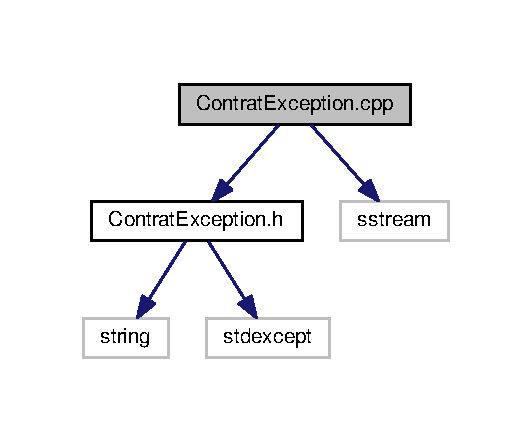
\includegraphics[width=255pt]{ContratException_8cpp__incl}
\end{center}
\end{figure}


\subsection{Detailed Description}
Implantation de la classe \hyperlink{classContratException}{Contrat\+Exception} et de ses héritiers. 

\begin{DoxyAuthor}{Author}
administrateur 
\end{DoxyAuthor}

\hypertarget{ContratException_8h}{}\section{Contrat\+Exception.\+h File Reference}
\label{ContratException_8h}\index{Contrat\+Exception.\+h@{Contrat\+Exception.\+h}}


Fichier contenant la déclaration de la classe \hyperlink{classContratException}{Contrat\+Exception} et de ses héritiers.  


{\ttfamily \#include $<$string$>$}\\*
{\ttfamily \#include $<$stdexcept$>$}\\*
Include dependency graph for Contrat\+Exception.\+h\+:\nopagebreak
\begin{figure}[H]
\begin{center}
\leavevmode
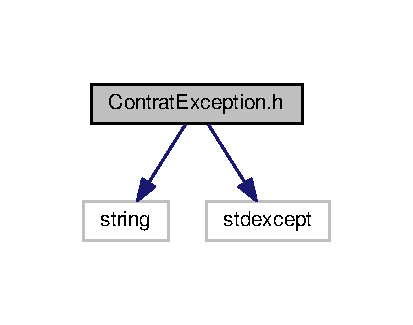
\includegraphics[width=198pt]{ContratException_8h__incl}
\end{center}
\end{figure}
This graph shows which files directly or indirectly include this file\+:\nopagebreak
\begin{figure}[H]
\begin{center}
\leavevmode
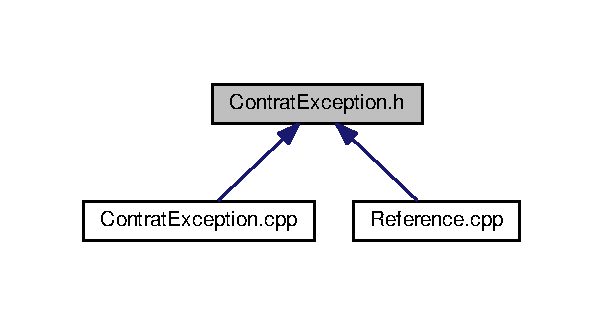
\includegraphics[width=289pt]{ContratException_8h__dep__incl}
\end{center}
\end{figure}
\subsection*{Classes}
\begin{DoxyCompactItemize}
\item 
class \hyperlink{classContratException}{Contrat\+Exception}
\begin{DoxyCompactList}\small\item\em Classe de base des exceptions de contrat. \end{DoxyCompactList}\item 
class \hyperlink{classAssertionException}{Assertion\+Exception}
\begin{DoxyCompactList}\small\item\em Classe pour la gestion des erreurs d\textquotesingle{}assertion. \end{DoxyCompactList}\item 
class \hyperlink{classPreconditionException}{Precondition\+Exception}
\begin{DoxyCompactList}\small\item\em Classe pour la gestion des erreurs de précondition. \end{DoxyCompactList}\item 
class \hyperlink{classPostconditionException}{Postcondition\+Exception}
\begin{DoxyCompactList}\small\item\em Classe pour la gestion des erreurs de postcondition. \end{DoxyCompactList}\item 
class \hyperlink{classInvariantException}{Invariant\+Exception}
\begin{DoxyCompactList}\small\item\em Classe pour la gestion des erreurs d\textquotesingle{}invariant. \end{DoxyCompactList}\end{DoxyCompactItemize}
\subsection*{Macros}
\begin{DoxyCompactItemize}
\item 
\#define {\bfseries I\+N\+V\+A\+R\+I\+A\+N\+TS}()~verifie\+Invariant()\hypertarget{ContratException_8h_a52dddc2c198c58b53b201c313934e40c}{}\label{ContratException_8h_a52dddc2c198c58b53b201c313934e40c}

\item 
\#define {\bfseries A\+S\+S\+E\+R\+T\+I\+ON}(f)~if (!(f)) throw \hyperlink{classAssertionException}{Assertion\+Exception}(\+\_\+\+\_\+\+F\+I\+L\+E\+\_\+\+\_\+,\+\_\+\+\_\+\+L\+I\+N\+E\+\_\+\+\_\+, \#f);\hypertarget{ContratException_8h_abe6e3e0ff48f8595570e6485b506a8c4}{}\label{ContratException_8h_abe6e3e0ff48f8595570e6485b506a8c4}

\item 
\#define {\bfseries P\+R\+E\+C\+O\+N\+D\+I\+T\+I\+ON}(f)~if (!(f)) throw \hyperlink{classPreconditionException}{Precondition\+Exception}(\+\_\+\+\_\+\+F\+I\+L\+E\+\_\+\+\_\+, \+\_\+\+\_\+\+L\+I\+N\+E\+\_\+\+\_\+, \#f);\hypertarget{ContratException_8h_acb3361bd87fc697a57b7286a9998c106}{}\label{ContratException_8h_acb3361bd87fc697a57b7286a9998c106}

\item 
\#define {\bfseries P\+O\+S\+T\+C\+O\+N\+D\+I\+T\+I\+ON}(f)~if (!(f)) throw \hyperlink{classPostconditionException}{Postcondition\+Exception}(\+\_\+\+\_\+\+F\+I\+L\+E\+\_\+\+\_\+, \+\_\+\+\_\+\+L\+I\+N\+E\+\_\+\+\_\+, \#f);\hypertarget{ContratException_8h_a438b75c0c77a1ce8d1e914f9f04ea548}{}\label{ContratException_8h_a438b75c0c77a1ce8d1e914f9f04ea548}

\item 
\#define {\bfseries I\+N\+V\+A\+R\+I\+A\+NT}(f)~if (!(f)) throw \hyperlink{classInvariantException}{Invariant\+Exception}(\+\_\+\+\_\+\+F\+I\+L\+E\+\_\+\+\_\+,\+\_\+\+\_\+\+L\+I\+N\+E\+\_\+\+\_\+, \#f);\hypertarget{ContratException_8h_a08f80155f47e05681c2b9bb9c5f6fffe}{}\label{ContratException_8h_a08f80155f47e05681c2b9bb9c5f6fffe}

\end{DoxyCompactItemize}


\subsection{Detailed Description}
Fichier contenant la déclaration de la classe \hyperlink{classContratException}{Contrat\+Exception} et de ses héritiers. 

\begin{DoxyAuthor}{Author}
administrateur 
\end{DoxyAuthor}

\hypertarget{Reference_8cpp}{}\section{Reference.\+cpp File Reference}
\label{Reference_8cpp}\index{Reference.\+cpp@{Reference.\+cpp}}


Implémentation de la classe Reference.  


{\ttfamily \#include \char`\"{}Reference.\+h\char`\"{}}\\*
{\ttfamily \#include $<$sstream$>$}\\*
{\ttfamily \#include \char`\"{}Contrat\+Exception.\+h\char`\"{}}\\*
Include dependency graph for Reference.\+cpp\+:\nopagebreak
\begin{figure}[H]
\begin{center}
\leavevmode
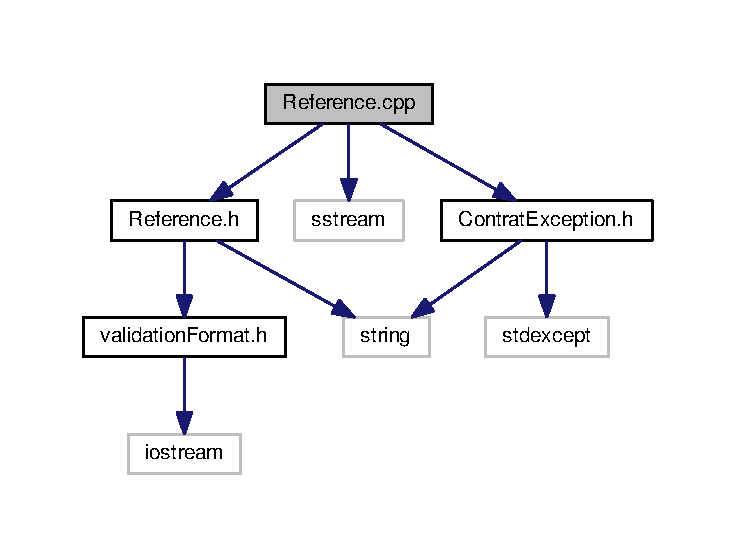
\includegraphics[width=350pt]{Reference_8cpp__incl}
\end{center}
\end{figure}
\subsection*{Namespaces}
\begin{DoxyCompactItemize}
\item 
 \hyperlink{namespacebiblio}{biblio}
\begin{DoxyCompactList}\small\item\em Constructeur qui crée un objet reference. \end{DoxyCompactList}\end{DoxyCompactItemize}


\subsection{Detailed Description}
Implémentation de la classe Reference. 

\begin{DoxyDate}{Date}
2019-\/02-\/22 
\end{DoxyDate}
\begin{DoxyAuthor}{Author}
Guillaume St-\/\+Georges 
\end{DoxyAuthor}

\hypertarget{Reference_8h}{}\section{Reference.\+h File Reference}
\label{Reference_8h}\index{Reference.\+h@{Reference.\+h}}


Prototype de la classe Reference.  


{\ttfamily \#include $<$string$>$}\\*
{\ttfamily \#include \char`\"{}validation\+Format.\+h\char`\"{}}\\*
Include dependency graph for Reference.\+h\+:\nopagebreak
\begin{figure}[H]
\begin{center}
\leavevmode
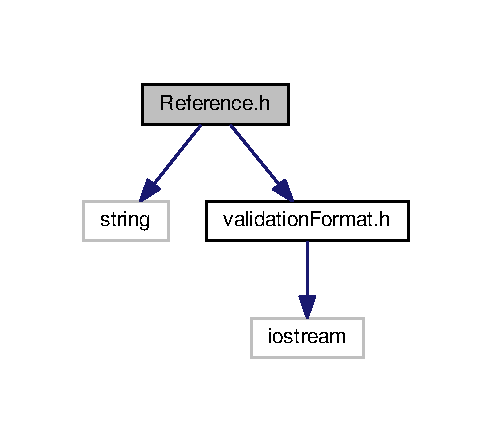
\includegraphics[width=236pt]{Reference_8h__incl}
\end{center}
\end{figure}
This graph shows which files directly or indirectly include this file\+:\nopagebreak
\begin{figure}[H]
\begin{center}
\leavevmode
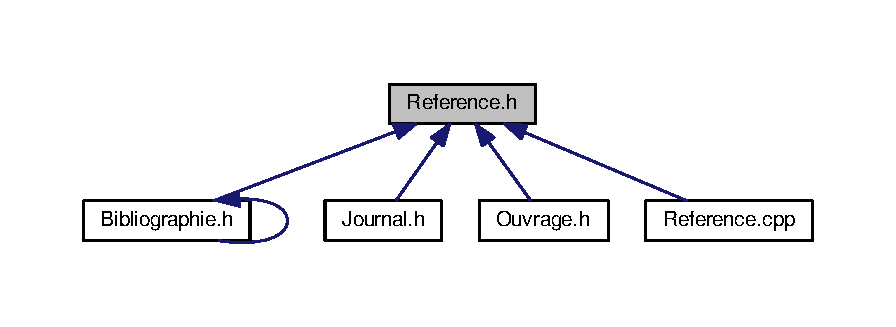
\includegraphics[width=350pt]{Reference_8h__dep__incl}
\end{center}
\end{figure}
\subsection*{Classes}
\begin{DoxyCompactItemize}
\item 
class \hyperlink{classbiblio_1_1Reference}{biblio\+::\+Reference}
\begin{DoxyCompactList}\small\item\em Classe \hyperlink{classbiblio_1_1Reference}{Reference} permettant de modéliser les objets reference. \end{DoxyCompactList}\end{DoxyCompactItemize}
\subsection*{Namespaces}
\begin{DoxyCompactItemize}
\item 
 \hyperlink{namespacebiblio}{biblio}
\begin{DoxyCompactList}\small\item\em Constructeur qui crée un objet reference. \end{DoxyCompactList}\end{DoxyCompactItemize}


\subsection{Detailed Description}
Prototype de la classe Reference. 

\begin{DoxyDate}{Date}
2019-\/02-\/22 
\end{DoxyDate}
\begin{DoxyAuthor}{Author}
Guillaume St-\/\+Georges 
\end{DoxyAuthor}

\hypertarget{validationFormat_8cpp}{}\section{validation\+Format.\+cpp File Reference}
\label{validationFormat_8cpp}\index{validation\+Format.\+cpp@{validation\+Format.\+cpp}}


Utilisation des fonctions de validation\+Format dans la classe Reference.  


{\ttfamily \#include \char`\"{}validation\+Format.\+h\char`\"{}}\\*
{\ttfamily \#include $<$string$>$}\\*
{\ttfamily \#include $<$cctype$>$}\\*
{\ttfamily \#include $<$stdexcept$>$}\\*
Include dependency graph for validation\+Format.\+cpp\+:\nopagebreak
\begin{figure}[H]
\begin{center}
\leavevmode
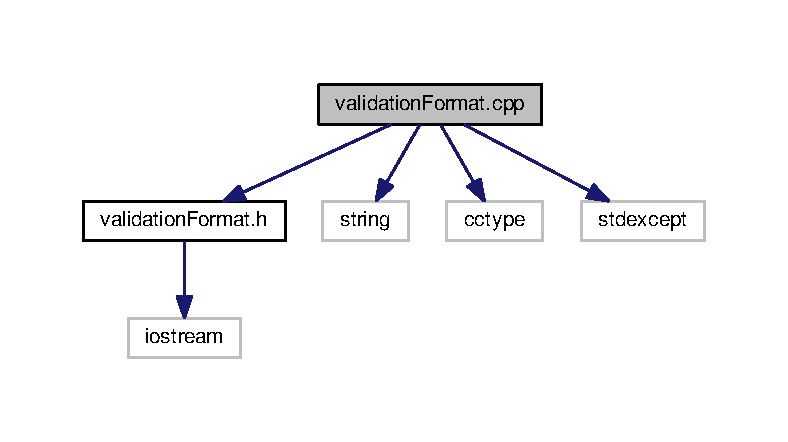
\includegraphics[width=350pt]{validationFormat_8cpp__incl}
\end{center}
\end{figure}
\subsection*{Functions}
\begin{DoxyCompactItemize}
\item 
bool \hyperlink{validationFormat_8cpp_ab3d93e73408df98688844f00a8cdce58}{util\+::valider\+Format\+Nom} (const std\+::string \&p\+\_\+nom)
\item 
bool \hyperlink{validationFormat_8cpp_a21c007029e2e42ca8c8daab00517069b}{util\+::valider\+Code\+Issn} (const std\+::string \&p\+\_\+issn)
\item 
bool \hyperlink{validationFormat_8cpp_a0955ea98068f9537dfb0d7fd66f10860}{util\+::valider\+Code\+Isbn} (const std\+::string \&p\+\_\+isbn)
\end{DoxyCompactItemize}


\subsection{Detailed Description}
Utilisation des fonctions de validation\+Format dans la classe Reference. 

\begin{DoxyDate}{Date}
2019-\/02-\/28 
\end{DoxyDate}
\begin{DoxyAuthor}{Author}
Guillaume St-\/\+Georges 
\end{DoxyAuthor}


\subsection{Function Documentation}
\index{validation\+Format.\+cpp@{validation\+Format.\+cpp}!valider\+Code\+Isbn@{valider\+Code\+Isbn}}
\index{valider\+Code\+Isbn@{valider\+Code\+Isbn}!validation\+Format.\+cpp@{validation\+Format.\+cpp}}
\subsubsection[{\texorpdfstring{valider\+Code\+Isbn(const std\+::string \&p\+\_\+isbn)}{validerCodeIsbn(const std::string &p_isbn)}}]{\setlength{\rightskip}{0pt plus 5cm}bool util\+::valider\+Code\+Isbn (
\begin{DoxyParamCaption}
\item[{const std\+::string \&}]{p\+\_\+isbn}
\end{DoxyParamCaption}
)}\hypertarget{validationFormat_8cpp_file_a0955ea98068f9537dfb0d7fd66f10860}{}\label{validationFormat_8cpp_file_a0955ea98068f9537dfb0d7fd66f10860}

\begin{DoxyParams}[1]{Parameters}
\mbox{\tt in}  & {\em p\+\_\+isbn} & \\
\hline
\end{DoxyParams}
\begin{DoxyReturn}{Returns}
True/\+False La validité du code I\+S\+BN 
\end{DoxyReturn}
\index{validation\+Format.\+cpp@{validation\+Format.\+cpp}!valider\+Code\+Issn@{valider\+Code\+Issn}}
\index{valider\+Code\+Issn@{valider\+Code\+Issn}!validation\+Format.\+cpp@{validation\+Format.\+cpp}}
\subsubsection[{\texorpdfstring{valider\+Code\+Issn(const std\+::string \&p\+\_\+issn)}{validerCodeIssn(const std::string &p_issn)}}]{\setlength{\rightskip}{0pt plus 5cm}bool util\+::valider\+Code\+Issn (
\begin{DoxyParamCaption}
\item[{const std\+::string \&}]{p\+\_\+issn}
\end{DoxyParamCaption}
)}\hypertarget{validationFormat_8cpp_file_a21c007029e2e42ca8c8daab00517069b}{}\label{validationFormat_8cpp_file_a21c007029e2e42ca8c8daab00517069b}

\begin{DoxyParams}[1]{Parameters}
\mbox{\tt in}  & {\em p\+\_\+issn} & Le code I\+S\+SN \\
\hline
\end{DoxyParams}
\begin{DoxyReturn}{Returns}
True/\+False La validité du code I\+S\+SN 
\end{DoxyReturn}
\index{validation\+Format.\+cpp@{validation\+Format.\+cpp}!valider\+Format\+Nom@{valider\+Format\+Nom}}
\index{valider\+Format\+Nom@{valider\+Format\+Nom}!validation\+Format.\+cpp@{validation\+Format.\+cpp}}
\subsubsection[{\texorpdfstring{valider\+Format\+Nom(const std\+::string \&p\+\_\+nom)}{validerFormatNom(const std::string &p_nom)}}]{\setlength{\rightskip}{0pt plus 5cm}bool util\+::valider\+Format\+Nom (
\begin{DoxyParamCaption}
\item[{const std\+::string \&}]{p\+\_\+nom}
\end{DoxyParamCaption}
)}\hypertarget{validationFormat_8cpp_file_ab3d93e73408df98688844f00a8cdce58}{}\label{validationFormat_8cpp_file_ab3d93e73408df98688844f00a8cdce58}

\begin{DoxyParams}{Parameters}
{\em p\+\_\+nom} & Nom d\textquotesingle{}un nom \\
\hline
\end{DoxyParams}
\begin{DoxyReturn}{Returns}
True/\+False La validité du format du nom 
\end{DoxyReturn}

\hypertarget{validationFormat_8h}{}\section{validation\+Format.\+h File Reference}
\label{validationFormat_8h}\index{validation\+Format.\+h@{validation\+Format.\+h}}


Appel des fonctions de validation format.  


{\ttfamily \#include $<$iostream$>$}\\*
Include dependency graph for validation\+Format.\+h\+:\nopagebreak
\begin{figure}[H]
\begin{center}
\leavevmode
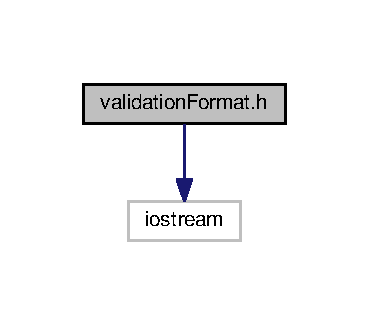
\includegraphics[width=177pt]{validationFormat_8h__incl}
\end{center}
\end{figure}
This graph shows which files directly or indirectly include this file\+:\nopagebreak
\begin{figure}[H]
\begin{center}
\leavevmode
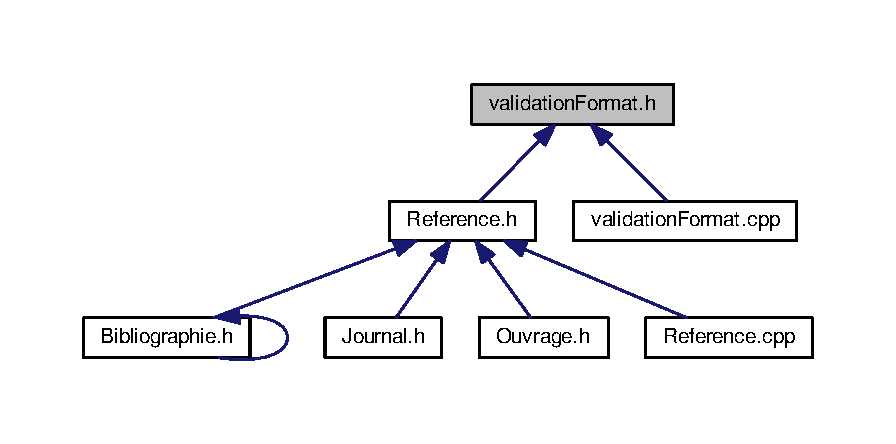
\includegraphics[width=350pt]{validationFormat_8h__dep__incl}
\end{center}
\end{figure}
\subsection*{Functions}
\begin{DoxyCompactItemize}
\item 
bool \hyperlink{validationFormat_8cpp_ab3d93e73408df98688844f00a8cdce58}{util\+::valider\+Format\+Nom} (const std\+::string \&p\+\_\+nom)
\item 
bool \hyperlink{validationFormat_8cpp_a21c007029e2e42ca8c8daab00517069b}{util\+::valider\+Code\+Issn} (const std\+::string \&p\+\_\+issn)
\item 
bool \hyperlink{validationFormat_8cpp_a0955ea98068f9537dfb0d7fd66f10860}{util\+::valider\+Code\+Isbn} (const std\+::string \&p\+\_\+isbn)
\end{DoxyCompactItemize}


\subsection{Detailed Description}
Appel des fonctions de validation format. 

\begin{DoxyDate}{Date}
2019-\/02-\/28 
\end{DoxyDate}
\begin{DoxyAuthor}{Author}
Guillaume St-\/\+Georges 
\end{DoxyAuthor}


\subsection{Function Documentation}
\index{validation\+Format.\+h@{validation\+Format.\+h}!valider\+Code\+Isbn@{valider\+Code\+Isbn}}
\index{valider\+Code\+Isbn@{valider\+Code\+Isbn}!validation\+Format.\+h@{validation\+Format.\+h}}
\subsubsection[{\texorpdfstring{valider\+Code\+Isbn(const std\+::string \&p\+\_\+isbn)}{validerCodeIsbn(const std::string &p_isbn)}}]{\setlength{\rightskip}{0pt plus 5cm}bool util\+::valider\+Code\+Isbn (
\begin{DoxyParamCaption}
\item[{const std\+::string \&}]{p\+\_\+isbn}
\end{DoxyParamCaption}
)}\hypertarget{validationFormat_8cpp_file_a0955ea98068f9537dfb0d7fd66f10860}{}\label{validationFormat_8cpp_file_a0955ea98068f9537dfb0d7fd66f10860}

\begin{DoxyParams}[1]{Parameters}
\mbox{\tt in}  & {\em p\+\_\+isbn} & \\
\hline
\end{DoxyParams}
\begin{DoxyReturn}{Returns}
True/\+False La validité du code I\+S\+BN 
\end{DoxyReturn}
\index{validation\+Format.\+h@{validation\+Format.\+h}!valider\+Code\+Issn@{valider\+Code\+Issn}}
\index{valider\+Code\+Issn@{valider\+Code\+Issn}!validation\+Format.\+h@{validation\+Format.\+h}}
\subsubsection[{\texorpdfstring{valider\+Code\+Issn(const std\+::string \&p\+\_\+issn)}{validerCodeIssn(const std::string &p_issn)}}]{\setlength{\rightskip}{0pt plus 5cm}bool util\+::valider\+Code\+Issn (
\begin{DoxyParamCaption}
\item[{const std\+::string \&}]{p\+\_\+issn}
\end{DoxyParamCaption}
)}\hypertarget{validationFormat_8cpp_file_a21c007029e2e42ca8c8daab00517069b}{}\label{validationFormat_8cpp_file_a21c007029e2e42ca8c8daab00517069b}

\begin{DoxyParams}[1]{Parameters}
\mbox{\tt in}  & {\em p\+\_\+issn} & Le code I\+S\+SN \\
\hline
\end{DoxyParams}
\begin{DoxyReturn}{Returns}
True/\+False La validité du code I\+S\+SN 
\end{DoxyReturn}
\index{validation\+Format.\+h@{validation\+Format.\+h}!valider\+Format\+Nom@{valider\+Format\+Nom}}
\index{valider\+Format\+Nom@{valider\+Format\+Nom}!validation\+Format.\+h@{validation\+Format.\+h}}
\subsubsection[{\texorpdfstring{valider\+Format\+Nom(const std\+::string \&p\+\_\+nom)}{validerFormatNom(const std::string &p_nom)}}]{\setlength{\rightskip}{0pt plus 5cm}bool util\+::valider\+Format\+Nom (
\begin{DoxyParamCaption}
\item[{const std\+::string \&}]{p\+\_\+nom}
\end{DoxyParamCaption}
)}\hypertarget{validationFormat_8cpp_file_ab3d93e73408df98688844f00a8cdce58}{}\label{validationFormat_8cpp_file_ab3d93e73408df98688844f00a8cdce58}

\begin{DoxyParams}{Parameters}
{\em p\+\_\+nom} & Nom d\textquotesingle{}un nom \\
\hline
\end{DoxyParams}
\begin{DoxyReturn}{Returns}
True/\+False La validité du format du nom 
\end{DoxyReturn}

%--- End generated contents ---

% Index
\backmatter
\newpage
\phantomsection
\clearemptydoublepage
\addcontentsline{toc}{chapter}{Index}
\printindex

\end{document}
